\section{\texorpdfstring{Implementation of \schannel and other models for \MET+X analyses}{Implementation of \schannel and \tchannel models for MET+X analyses}}

In the studies to date, a fair number of different Monte Carlo tools have
been used to simulate signals.   In this Chapter, we make recommendations
and provide settings to promote uniformity in the simulations produced by
the collaborations.  These recommendations are based on the current
status of the available codes.   We also aim for simplicity, so that fewer
tools need be used if the theoretical quality does not suffer.


\subsection{Implementation of ``s-channel'' models for mono-jet signature}
\label{sec:monojet_implementation}

These models include those referred to as \modelDMV, \modelDMA, \modelDMS and
\modelDMP and discussed in Secs.~\ref{sec:monojet_V} and \ref{sec:monojet_scalar}.
The necessary simulations are geared for monojet analyses, i.e. those with a few jets and \MET{}.   In particular, the \MET{} spectrum depends upon the accurate simulation of parton radiation from the initial state.   For the \modelDMV and
\modelDMA models, we recommend \powheg \cite{Haisch:2013ata},
since it includes NLO corrections for these models.
The NLO corrections result in a substantial reduction
in the dependence on the choice of the renormalization and factorization
scale and hence the theoretical uncertainty on the signal prediction.
For the central choice of renormalization and factorization scales,
the NLO corrections also provide a minor enhancement in the cross section.\footnote{\spinzero and \spinone 
mediator models will also be provided 
in the near future to the same precision in \madgraph~\cite{Alwall:1405.0301}.}

For the \modelDMS and \modelDMP models, the lowest order process
already involves a one-loop amplitude in QCD.
Because of this complexity, NLO calculations for these signals do not
yet exist with a parton shower interface.
For these spin-0 mediators in the mono-jet final state,
the top-quark loop is the most important consideration.
The matrix element implementation of the \schannel spin-0 mediated DM production is available in \mcfm~\cite{Fox:2012ru,Harris:2014hga} and \powheg~\cite{Haisch:2015ioa} with the full top-loop calculation at LO.
The \powheg and \mcfm implementations include the finite
top quark mass dependence for DM pair production with 1 parton at LO.
For consistency with the spin-1 generation, we recommend using \powheg.

Here, we document some specific settings needed to run the \powheg 
generation for the Dark Matter models. POWHEG parameter cards for all models
can be found on the Forum SVN
repository~\cite{ForumSVN_DMA, ForumSVN_DMV, ForumSVN_DMS_tloop, ForumSVN_DMP_tloop}.

\subsubsection{\powheg configuration for DM models}

The lastest \powheg release is available for download using the
instructions at
\url{http://powhegbox.mib.infn.it/}.   The forum recommends
using at least version \texttt{x.xxx}.

\begin{itemize}

\item \powheg can generate either unweighted (uniformly--weighted) or
weighted events.  
The relevant keywords in the input card are \bornsuppfact and \bornktmin. 

\begin{enumerate}
\item unweighted events: %keywords

\bornsuppfact: negative or absent\\
\bornktmin <PT>

This runs the program in the most straightforward way,
but it is likely not the more convenient choice, as will be
explained below. \powheg will generate unweighted events using a sharp
lower cut (with value \texttt{PT}) on the leading-jet \pT. Since this is a
generation cut, the user must check that the choice of \bornktmin
does not change the cross section for signal events passing analysis selections.
It is good practice to use as a value in the input card a
transverse momentum 10-20\% smaller than the final analysis selection
on \MET{}, and check that the final result is independent, by exploring an even
smaller value of \bornktmin. The drawback of using this mode is that
it is difficult to populate well, and in a single run, both the low-\pT
region as well as the high-\pT tail.

\item weighted events: %keywords

\bornsuppfact <PTS>\\
\bornktmin <PT>

\powheg will now produce weighted events, thereby allowing to generate
a single sample that provides sufficient statistics in all signal
regions. Events are still generated with a sharp lower cut set by
\bornktmin, but the \bornsuppfact parameter is used to set the event
suppression factor according to


\begin{equation}
F(\kT)=\frac{\kT^2}{\kT^2+\bornsuppfact^2} \;.
\end{equation}

In this way, the events at, for instance, low \MET, are suppressed
but receive higher weight, which ensures at the same time higher
statistics at high \MET. We recommend to set \bornsuppfact to 1000.

The \bornktmin parameter can be used in conjunction with \bornsuppfact to suppress the low \MET region
even further.  It is recommended to set \bornktmin to one--half the value of
the lowest \MET selection. For instance,  for the event selection used in the
CMS/ATLAS monojet analyses, assuming the lowest \MET region being defined above 300\,GeV, the proposed value for
\bornktmin is 150.  However, this parameter should be set keeping in
mind the event selection of all the analyses that will use these
signal samples, and hence a threshold lower than 150 may be required.

\end{enumerate}



%\begin{itemize}

\item Remove the \runningwidth keyword, or set it to 0, which is the
  default value. Running with fixed widths is the recommended
  option. Although there are limitations, this is the more
  straightforward, simple and transparent option, and it was used for these
  Forum studies. 

  %  While not recommended,
  The alternative, a running width for the
  propagator of the \schannel mediator, can be selected by setting
  runningwidth to 1. In this case the denominator of the mediator's
  propagator is modified:
  
\begin{equation*}
  Q^2 - M^2 + \complexi\,M\,\Gamma \to   Q^2 - M^2 + \complexi\,Q^2\,\frac{\Gamma}{M},
\end{equation*}
where $Q$ is the virtuality of the mediator, and $M$ and $\Gamma$ are
its mass and width respectively.  See Ref.~\cite{Bardin:1989qr} for
a discussion.

\item Set the parameters defining the bounds on the invariant mass of the Dark Matter pair, \masslow and \masshigh, to -1. In this way, \powheg will assign values internally. 
\item The minimal values for \ncallOne, \itmxOne, \ncallTwo, \itmxTwo are 250000, 5, 1000000, 5 for the vector model, respectively.
\item The minimal values for \ncallOne, \itmxOne, \ncallTwo, \itmxTwo are 100000, 5, 100000, 5 for the scalar top-loop model, respectively.
\item When NLO corrections are included (as for instance in the
  vector model), negative-weighted events could happen and should
  be kept in the event sample, hence \withnegweights should be set to
  1. If needed, their fraction can be decreased by setting \foldsci
  and \foldy to bigger value (2 for instance). \foldphi can be kept to
  1.
\item Since the scalar model with top-loop is computed as a leading order process, set \LOevents and \bornonly are set to 1 internally.
\item One should use the automatic calculation of systematic uncertainties associated with the choice of hard scale and PDFs as described in Section\,\ref{sec:TheoryUncertainties}.

\item \texttt{idDM} is the integer that identifies the DM particle in the Monte Carlo event record.  This should be chosen so that other tools can process the \powheg output properly.

\end{itemize}


\powheg in itself is not an event generator and must be interfaced with a tool that provides parton showering, hadronization, \textit{etc.}   For some time, a
\pythiaEight \cite{Sjostrand:2014zea} interface
has existed for \powheg.  The \pythiaEight runtime configuration is
the following:

\begin{verbatim}
POWHEG:veto = 1
POWHEG:pTdef = 1
POWHEG:emitted = 0
POWHEG:pTemt = 0
POWHEG:pThard = 0
POWHEG:vetoCount = 100
SpaceShower:pTmaxMatch = 2
TimeShower:pTmaxMatch = 2
\end{verbatim}
As always, it is recommended to use the latest \pythiaEight release,
available at \url{http://home.thep.lu.se/~torbjorn/Pythia.html}.
At the time of this report, the latest version is \texttt{8.209}.

\subsection{Implementation of models with matching}
\label{sec:monojet_parton_match}

For the models discussed in the previous section, it is important
to calculate the hard process as accurately as possible in QCD.
For many other signal models, the \MET{} signature depends more
upon the production and decay of the mediator.  Also, for some models,
no NLO+parton shower implementations currently exist.  In these cases,
one usually resorts to a LO+parton shower implementation, sometimes
supplemented by several LO processes matched with the parton shower.

Here, we consider the example of an EFT model produced in association
with up to 2 additional QCD partons.   A Monte Carlo sample based on
this model could be used to cross-check a similar \powheg sample, for example.
The methodology described here could also be used for the \tchannel model
discussed in Sec.~\ref{sec:monojet_t_channel},

For the calculation of tree-level, signal models, we recommend
\madgraph.
\madgraph provides a flexible and easy--to--use framework for implementing
new models via the {\sc FeynRules} package.
\madgraph can produce both LO and NLO calculations, though not all signal models
can be generated currently at NLO.\footnote{For truly NLO, matched samples, a different
  matching scheme would be used.}
The parton matching is performed in order to avoid double counting of the
partons from matrix elements and parton showering.
Several parton matching techniques are available.
Based on some comparative studies \,\cite{Alwall:0706.2569},
there is some advantage to using the CKKW-L matching scheme \cite{Lonnblad:2011xx}
implemented in \pythiaEight.  Alternatively, one can use the $k_T$-MLM scheme also
implemented in \pythiaEight.


\subsubsection{Generation of the LHE file}

The example presented here is a D5 EFT model, and
includes tree-level diagrams with $\chi\bar\chi$+0,1,2 partons.
The model is encapsulated as a UFO file in the SVN repository (ref here).
\madgraph, like \powheg, is not in itself and event generator, but must be interfaced
with an event generator through an LHE file.  The production of the LHE file proceeds
through setting the process parameters and the run parameters.

The process parameters are:
\begin{verbatim}
import model MODELNAME
generate p p > chi chi~ [QCD] @0
add process p p > chi chi~ j [QCD] @1
add process p p > chi chi~ j j [QCD] @2
\end{verbatim}

The runtime parameters are more numerous, and define the
collider properties, PDF sets, etc.   The specific parameters
needed for matching are, for example:
\begin{verbatim}
ickkw = 0
ktdurham = matching scale
dparameter = 0.4
dokt = T
ptj=20
drjj=0
mmjj=0
ptj1min=0
\end{verbatim}
For different kinds of matching, a different choice of \texttt{ickkw} and
related parameters would be made.


\subsubsection{Implementation of the CKKW-L matching}
\label{sec:match_implementation}


To illustrate the settings related to parton matching, the EFT D5 samples were generated with \madgraph version 2.2.2 and showered in \pythiaEight.201.

The \pythiaEight parameters for the CKKW-L $k_T$-merging scheme are:
\begin{verbatim}
Merging:ktType           = 1
Merging:TMS              = matching scale
1000022:all = chi chi~ 2 0 0 30.0 0.0 0.0 0.0 0.0 
1000022:isVisible = false
Merging:doKTMerging      = on
Merging:Process          = pp>{chi,1000022}{chi~ -1000022}
Merging:nJetMax          = 2
\end{verbatim}
The matching scales should be the same for the generation and parton showering.
In the model implementation, the particle data group ID \texttt{1000022} is used for weakly
interacting dark matter candidates.   Since this is a Majorana particle by default (with no
corresponding anti-particle), and the model produces a DM Dirac fermion, the particle properties
are changed accordingly.  Also, the DM mass is set to 30\,\gev.
The \texttt{Merging:Process} command specifies the lowest parton emission process generated in \madgraph and \texttt{Merging:nJetMax = 2} gives the maximum number of additional parton emissions with respect to the lowest parton emission process. 


 In general, it is desired to take the hard parton emissions from the matrix element generation in \madgraph and allow \pythiaEight to take care of soft emissions only. The transition between these two regimes is defined by the matching scale and its optimal value can be determined by studying the cross-section as a function of the number of jets (differential jet rates). The differential rates $\frac{dN_{i\to j}}{d \log_{10}(k_\textrm{cut})}$ give the number of events which pass from $i$ jets to $j$ jets as the $k_T$ value increases beyond $k_\textrm{cut}$. An optimal matching scale should lead to smooth differential jet rates.

 Two examples of differential jet rates, using matching scale 30\,\gev and 80\,\gev, from the EFT D5 sample generated as described in the previous section are given in Fig.\,\ref{fig:CKKW_D5_30} and \ref{fig:CKKW_D5_80}, respectively.
 Although a kink is visible around the matching scale value in both cases, the 80\,\gev scale leads to smoother distributions. 
 In order to find the optimal matching scale, additional samples with matching scale 50, 70, and 90\,\gev are generated as well and a detailed comparison of the differential jet rates close to the transition region is shown in Fig.\,\ref{fig:CKKW_D5_zoom}.
 The largest differences among the samples are visible for the $1\rightarrow2$ jets transition where the 30\,\gev and 50\,\gev scale lead to a drop of the rates around the matching scale values. On the contrary, there is a hint of an increased rate around the matching scale value in the sample generated with the 90\,\gev scale. Therefore, we recommend to use 80\,\gev as the baseline matching scale.


 \begin{figure}[h!]
 	\centering  
 	\subfloat[$1\rightarrow2$ jets]{%
 		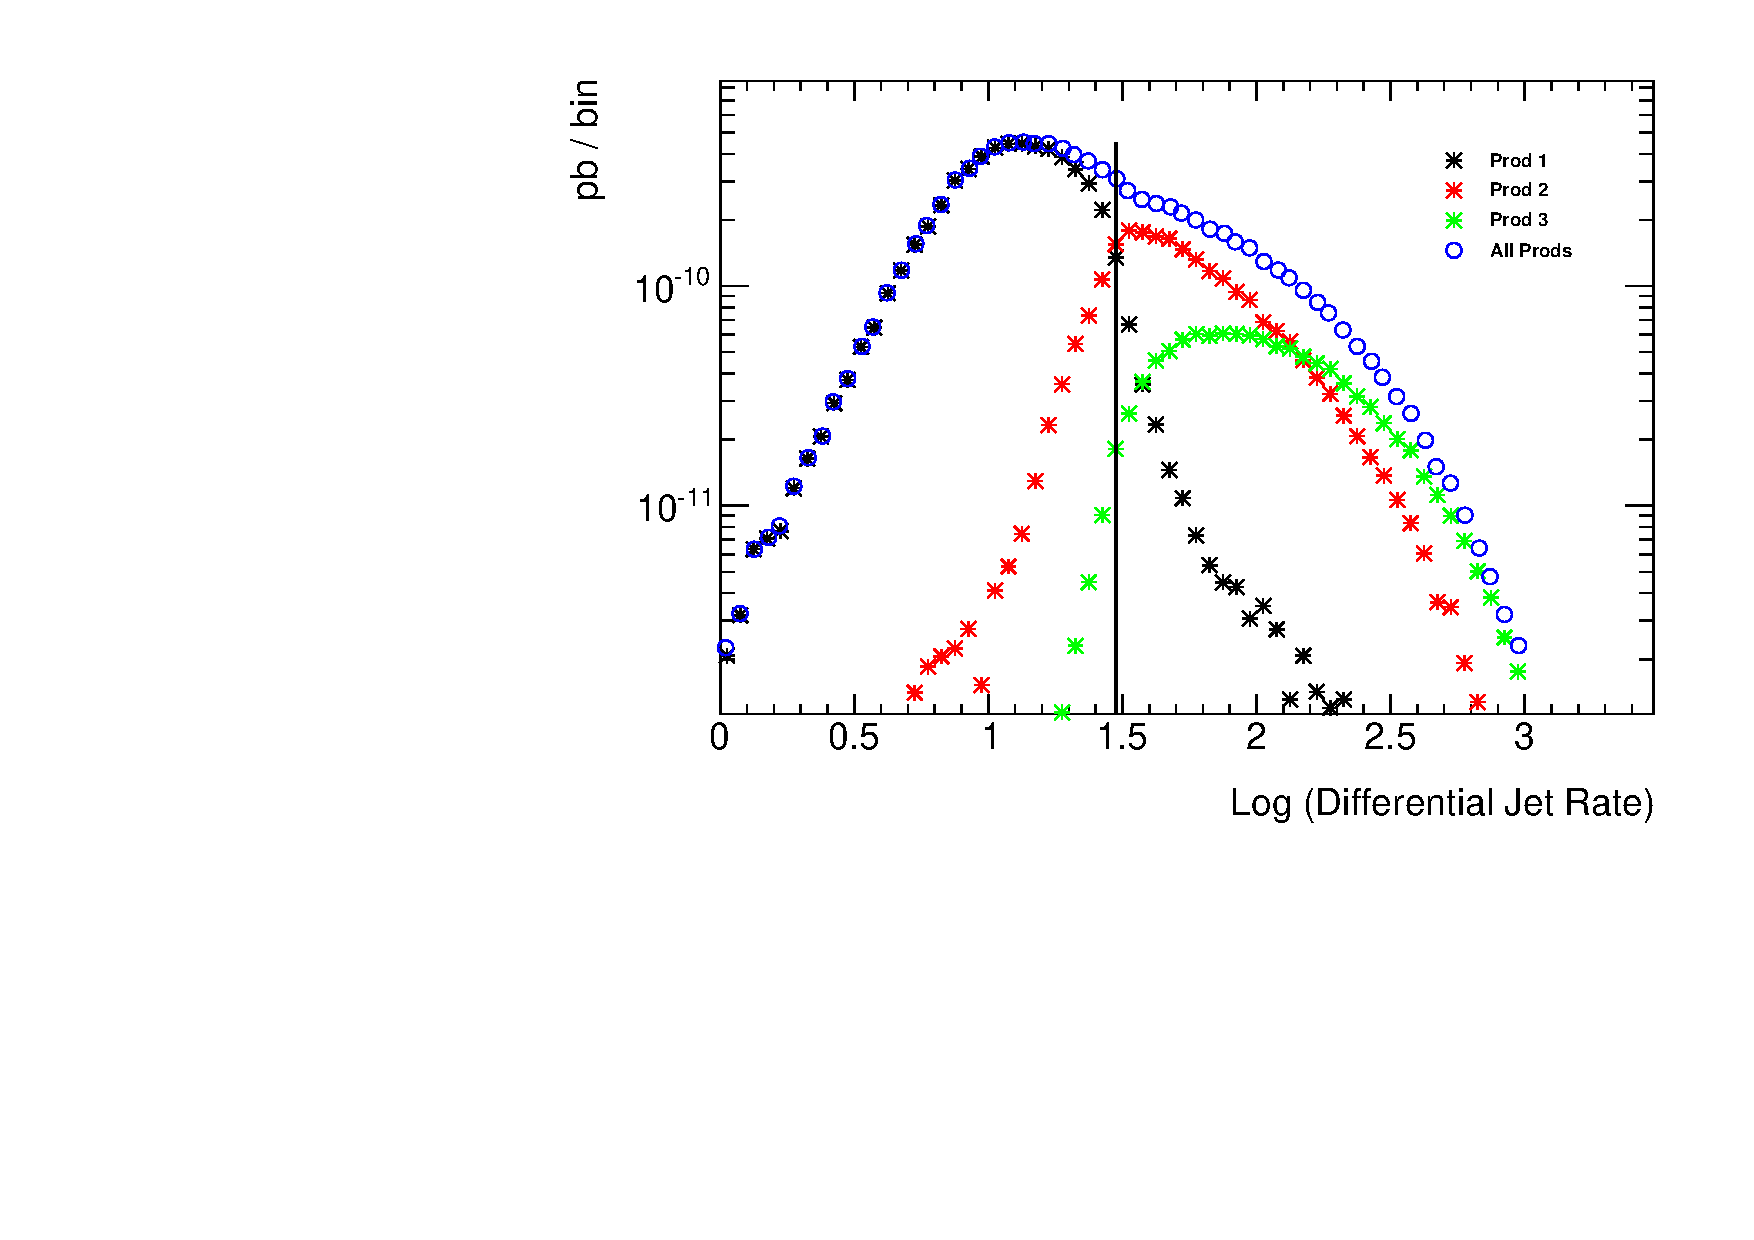
\includegraphics[width=0.45\linewidth]{figures/monojet_appendix/HistoJet1to2_30.pdf}
 	}
 	\hfill
 	\subfloat[$2\rightarrow3$ jets]{%
 		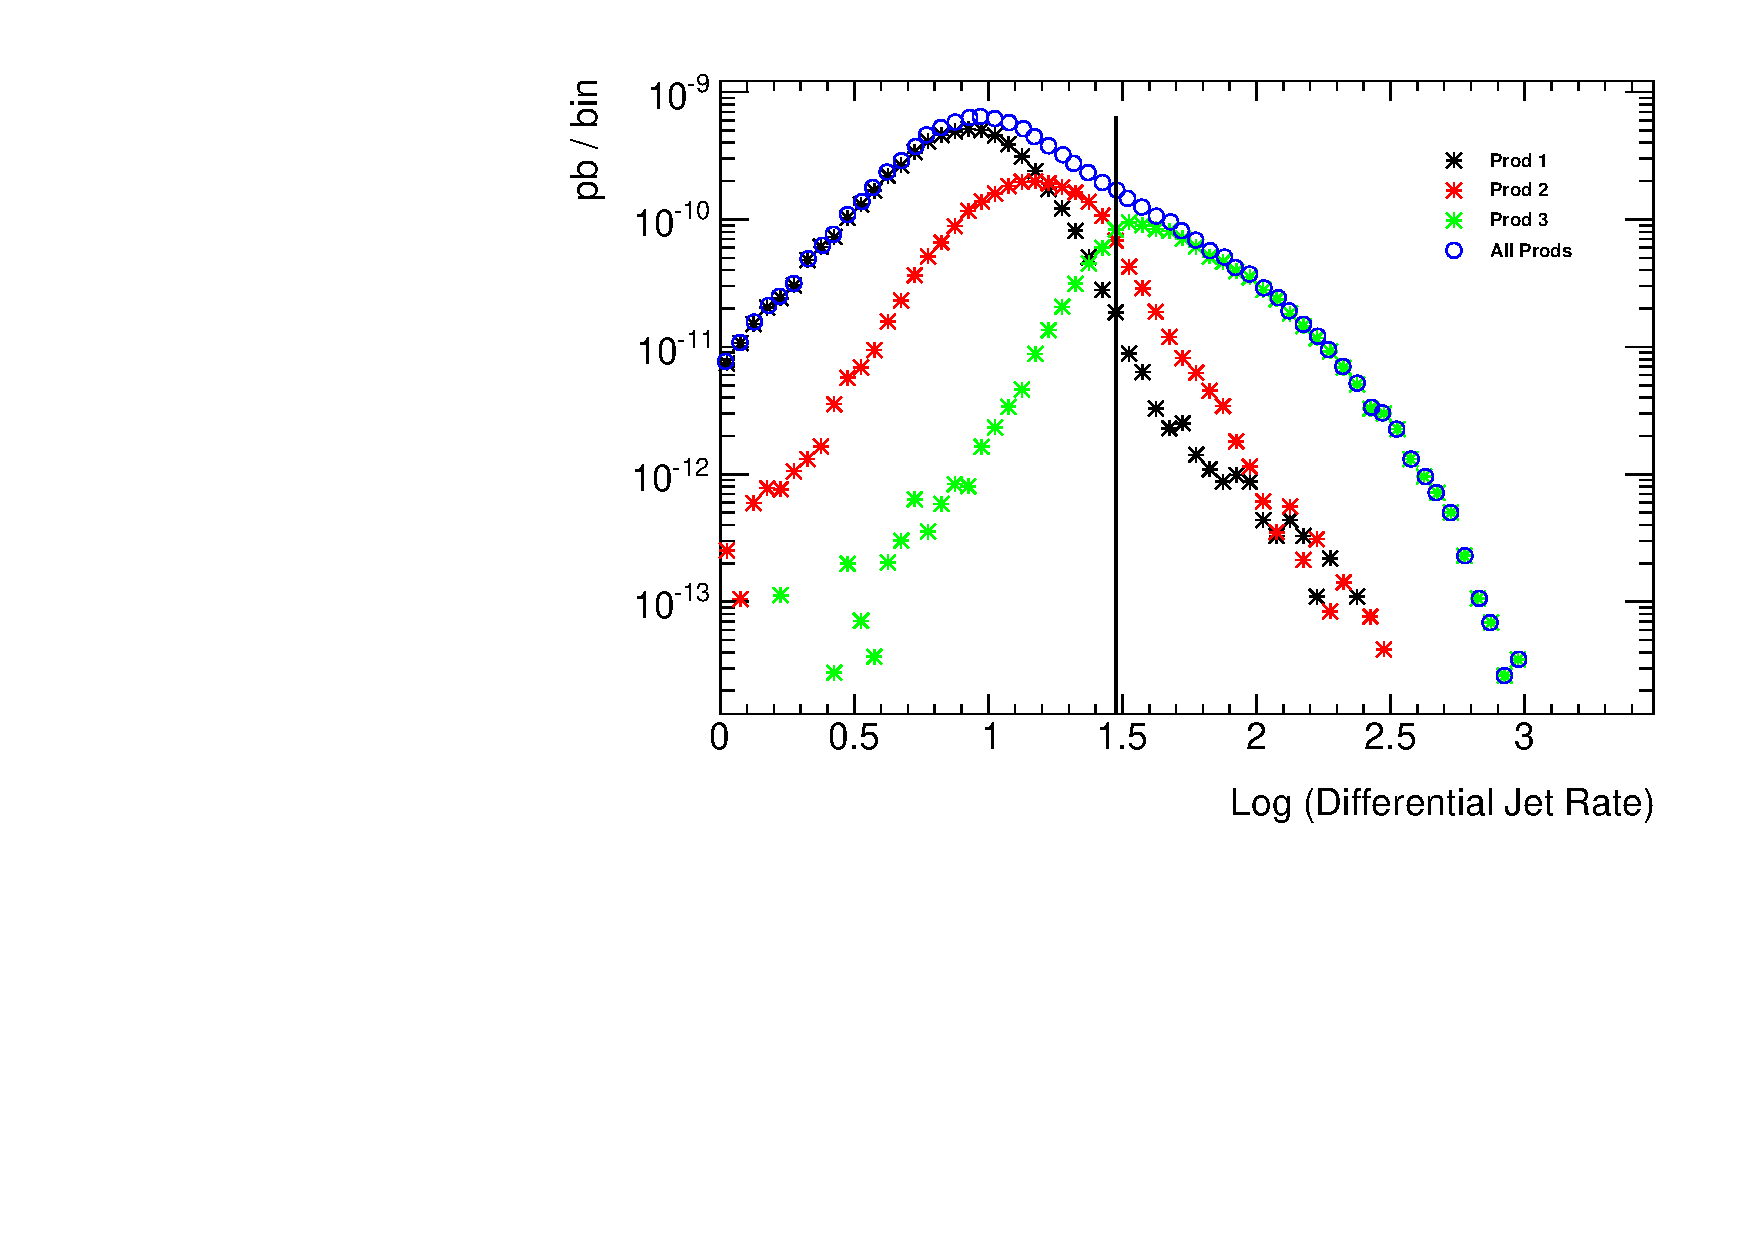
\includegraphics[width=0.45\linewidth]{figures/monojet_appendix/HistoJet2to3_30.pdf}
 	}
 	\hfill
 	\subfloat[$3\rightarrow4$ jets]{%
 		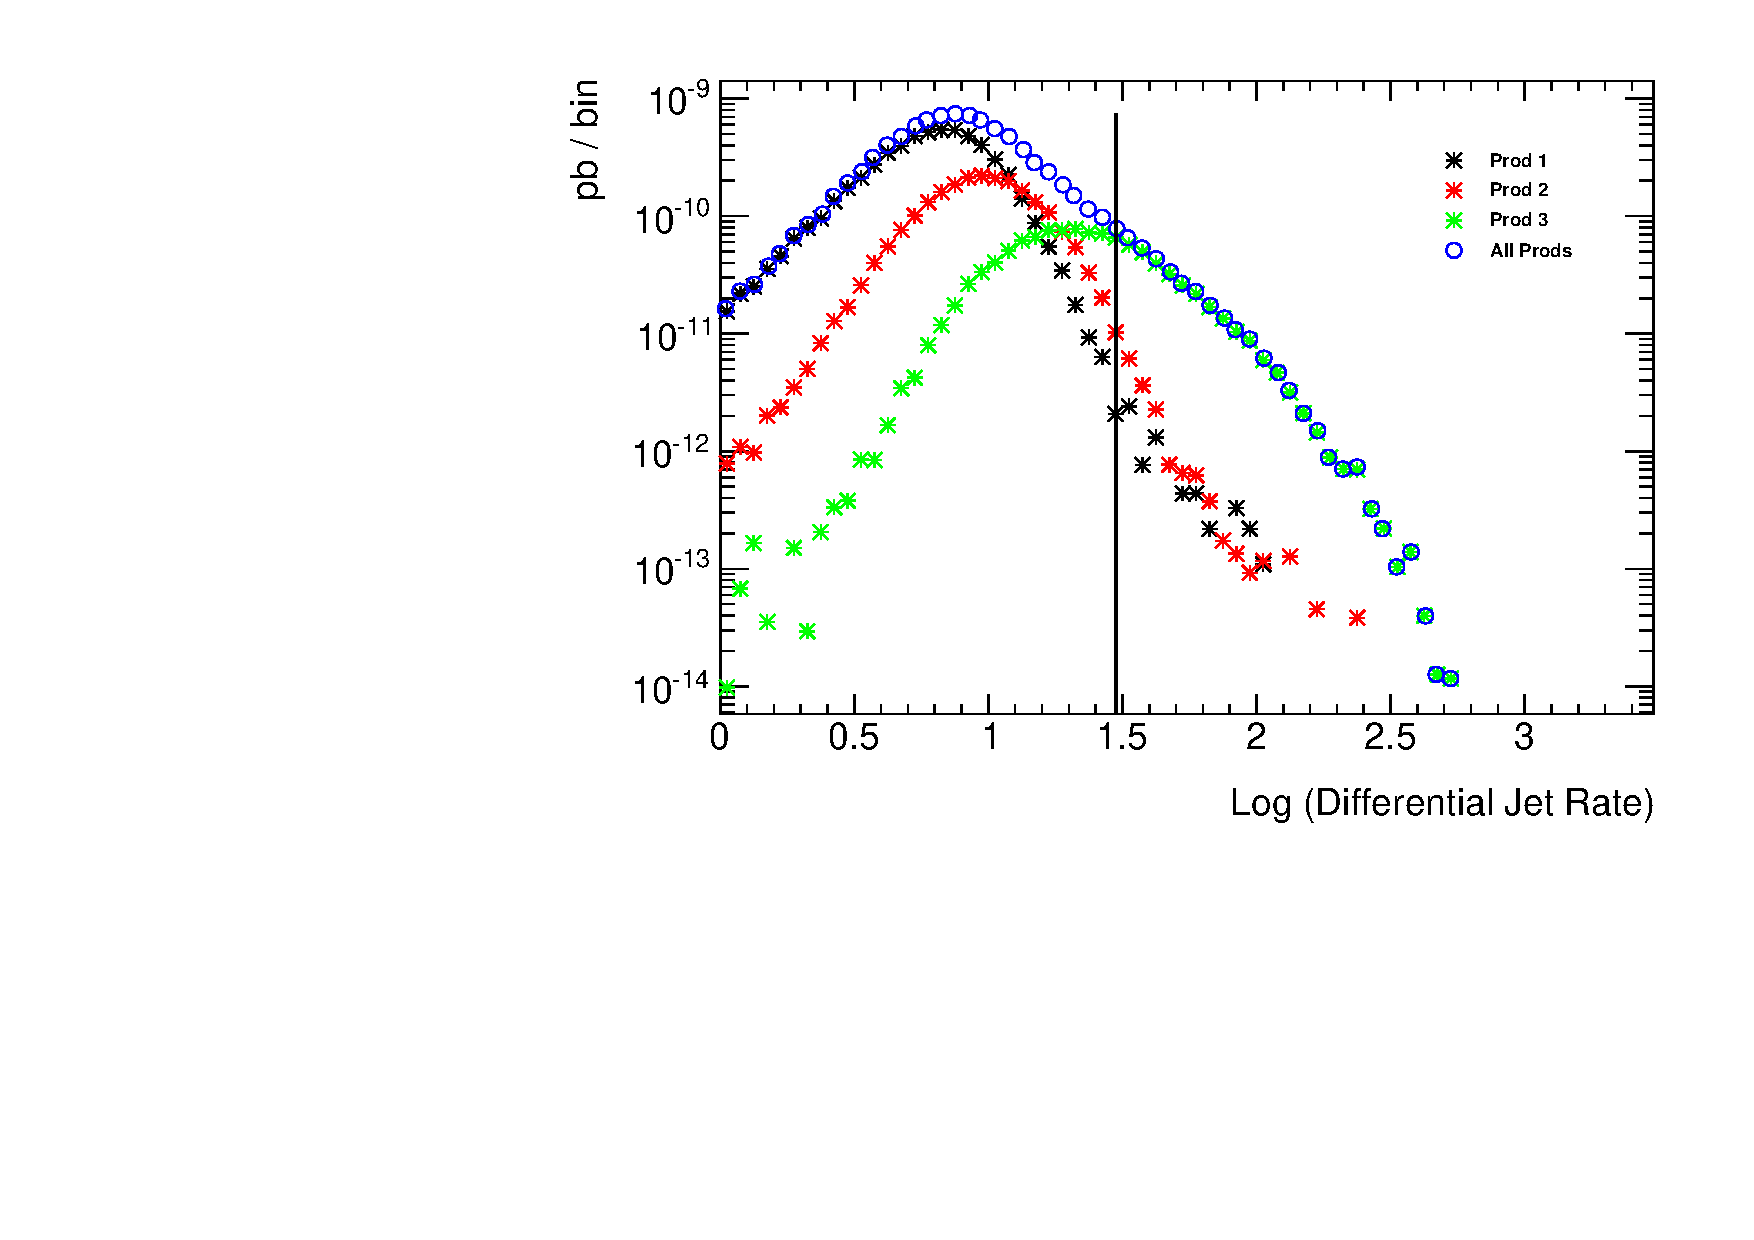
\includegraphics[width=0.45\linewidth]{figures/monojet_appendix/HistoJet3to4_30.pdf}
 	}
 	\hfill
 	\subfloat[$4\rightarrow5$ jets]{%
 		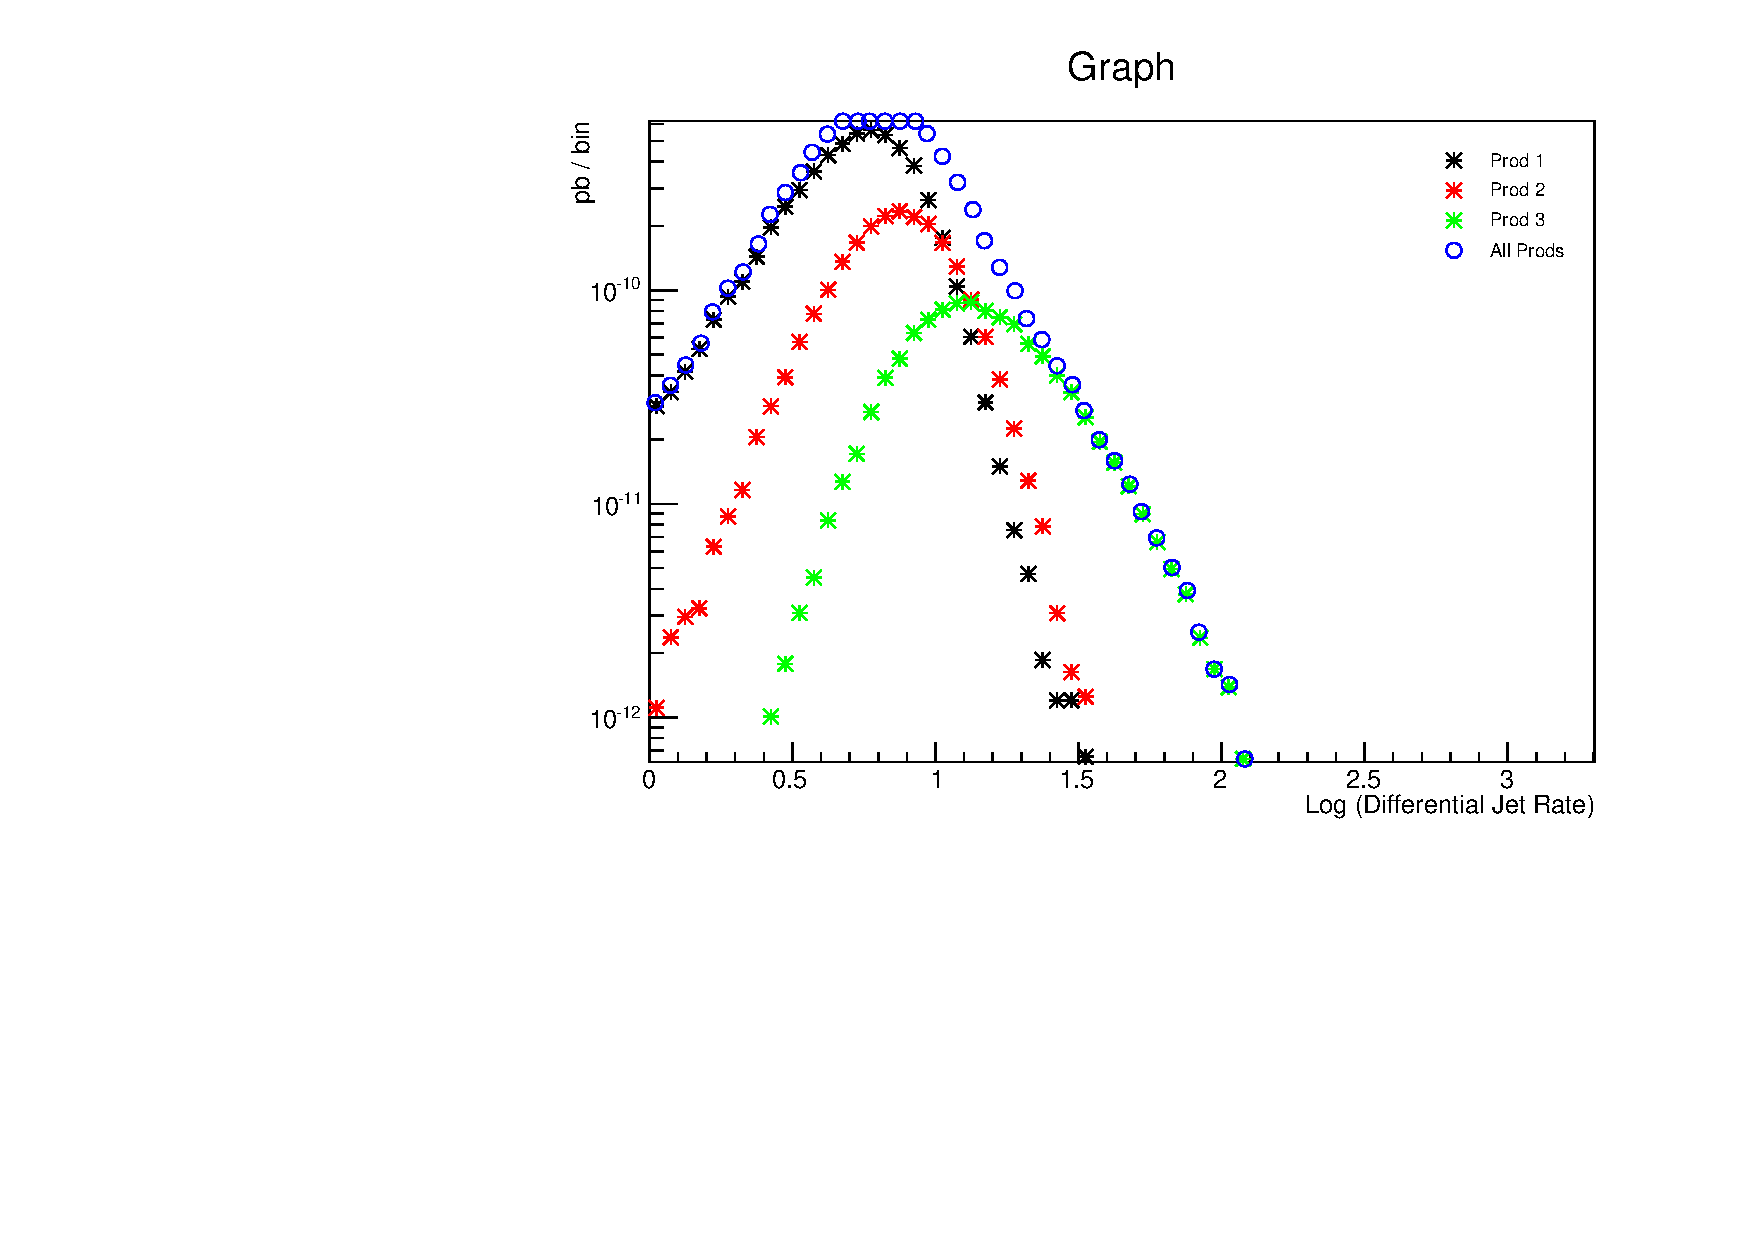
\includegraphics[width=0.45\linewidth]{figures/monojet_appendix/HistoJet4to5_30.pdf}
 	}
 	\caption{Distributions of differential jet rates $\frac{dN_{i\to j}}{d \log_{10}(k_\textrm{cut})}$ for EFT D5 sample with CKKW-L matching scale at 30\,\gev. The 0-, 1- and 2-parton emission samples are generated separately and indicated in the plots as Prod 1, Prod 2 and Prod 3, respectively. A vertical line is drawn at the matching scale.}
 	\label{fig:CKKW_D5_30}
 \end{figure}


 \begin{figure}[h!]
 	\centering  
 	\subfloat[$1\rightarrow2$ jets]{%
 		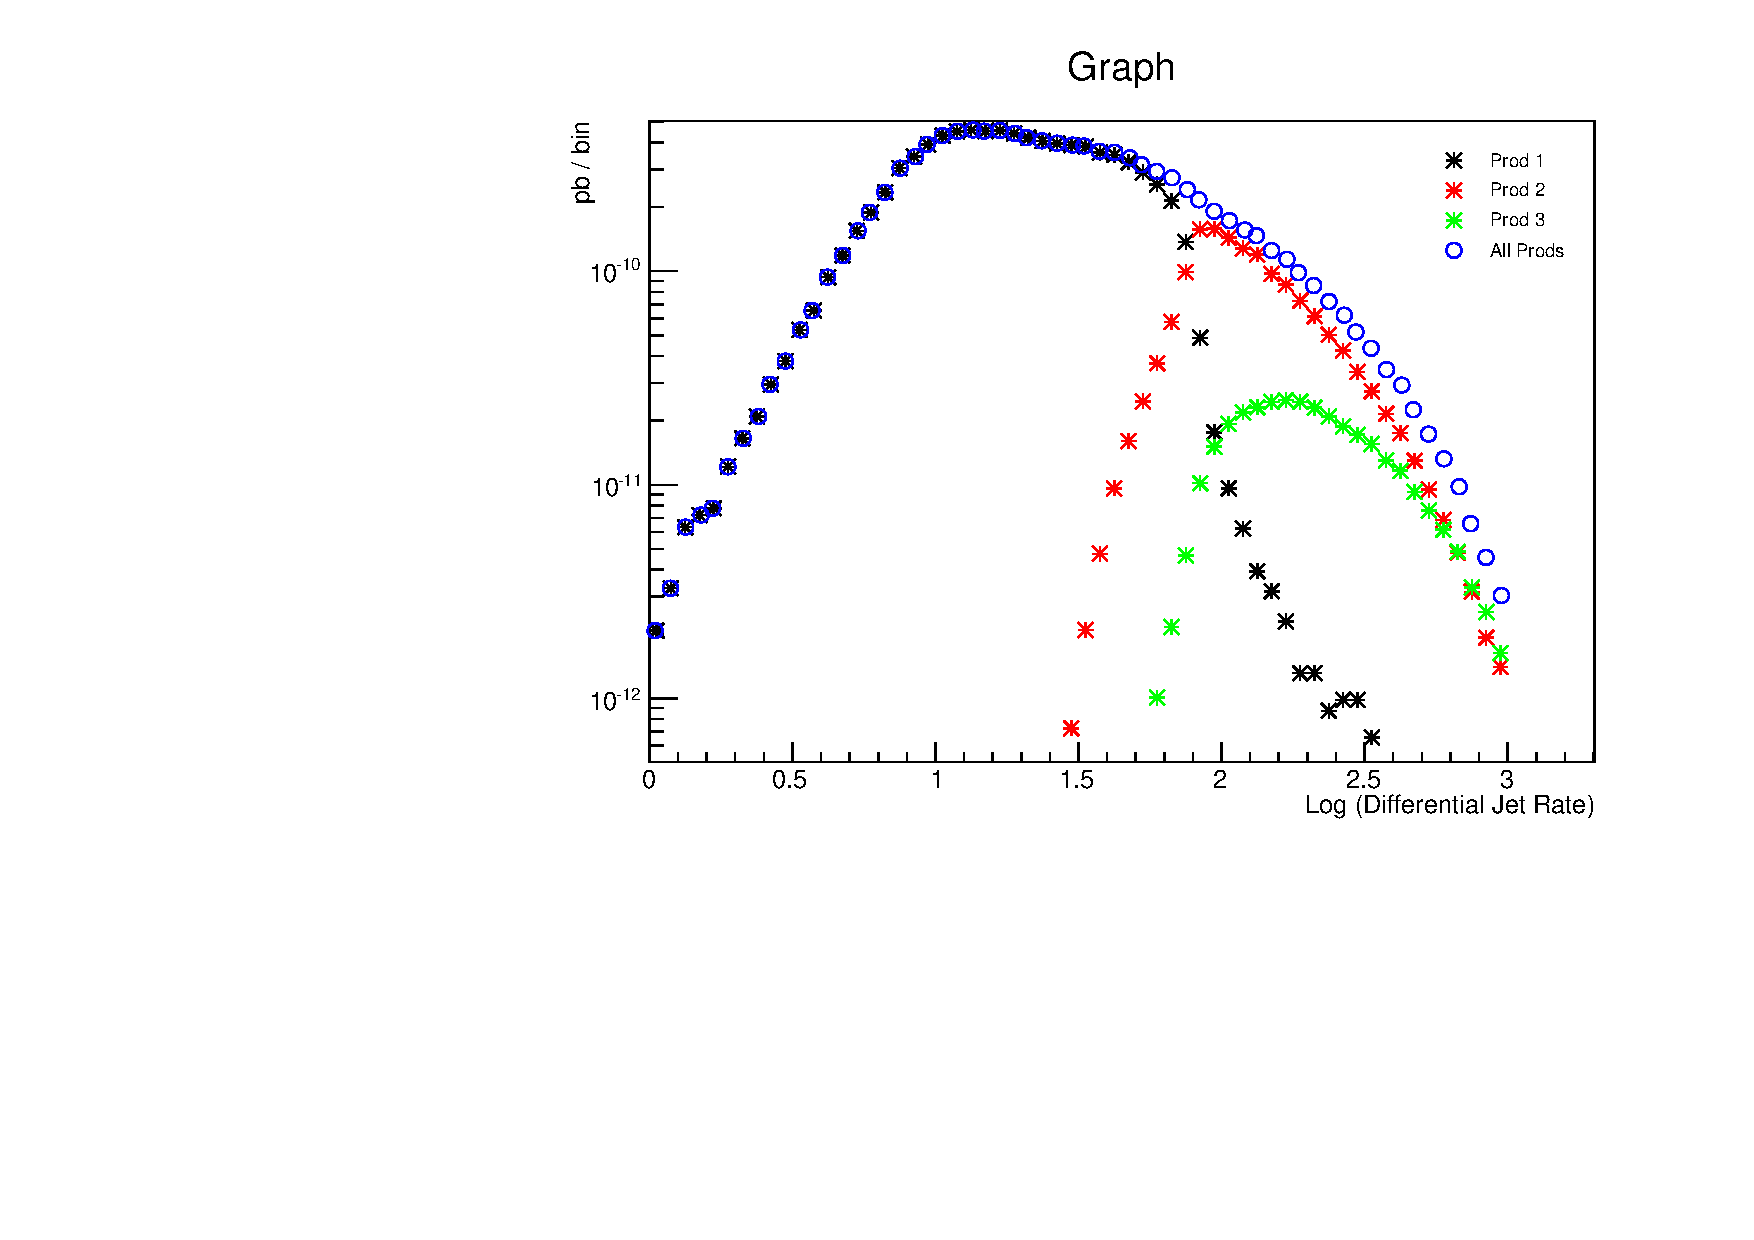
\includegraphics[width=0.45\linewidth]{figures/monojet_appendix/HistoJet1to2_80.pdf}
 	}
 	\hfill
 	\subfloat[$2\rightarrow3$ jets]{%
 		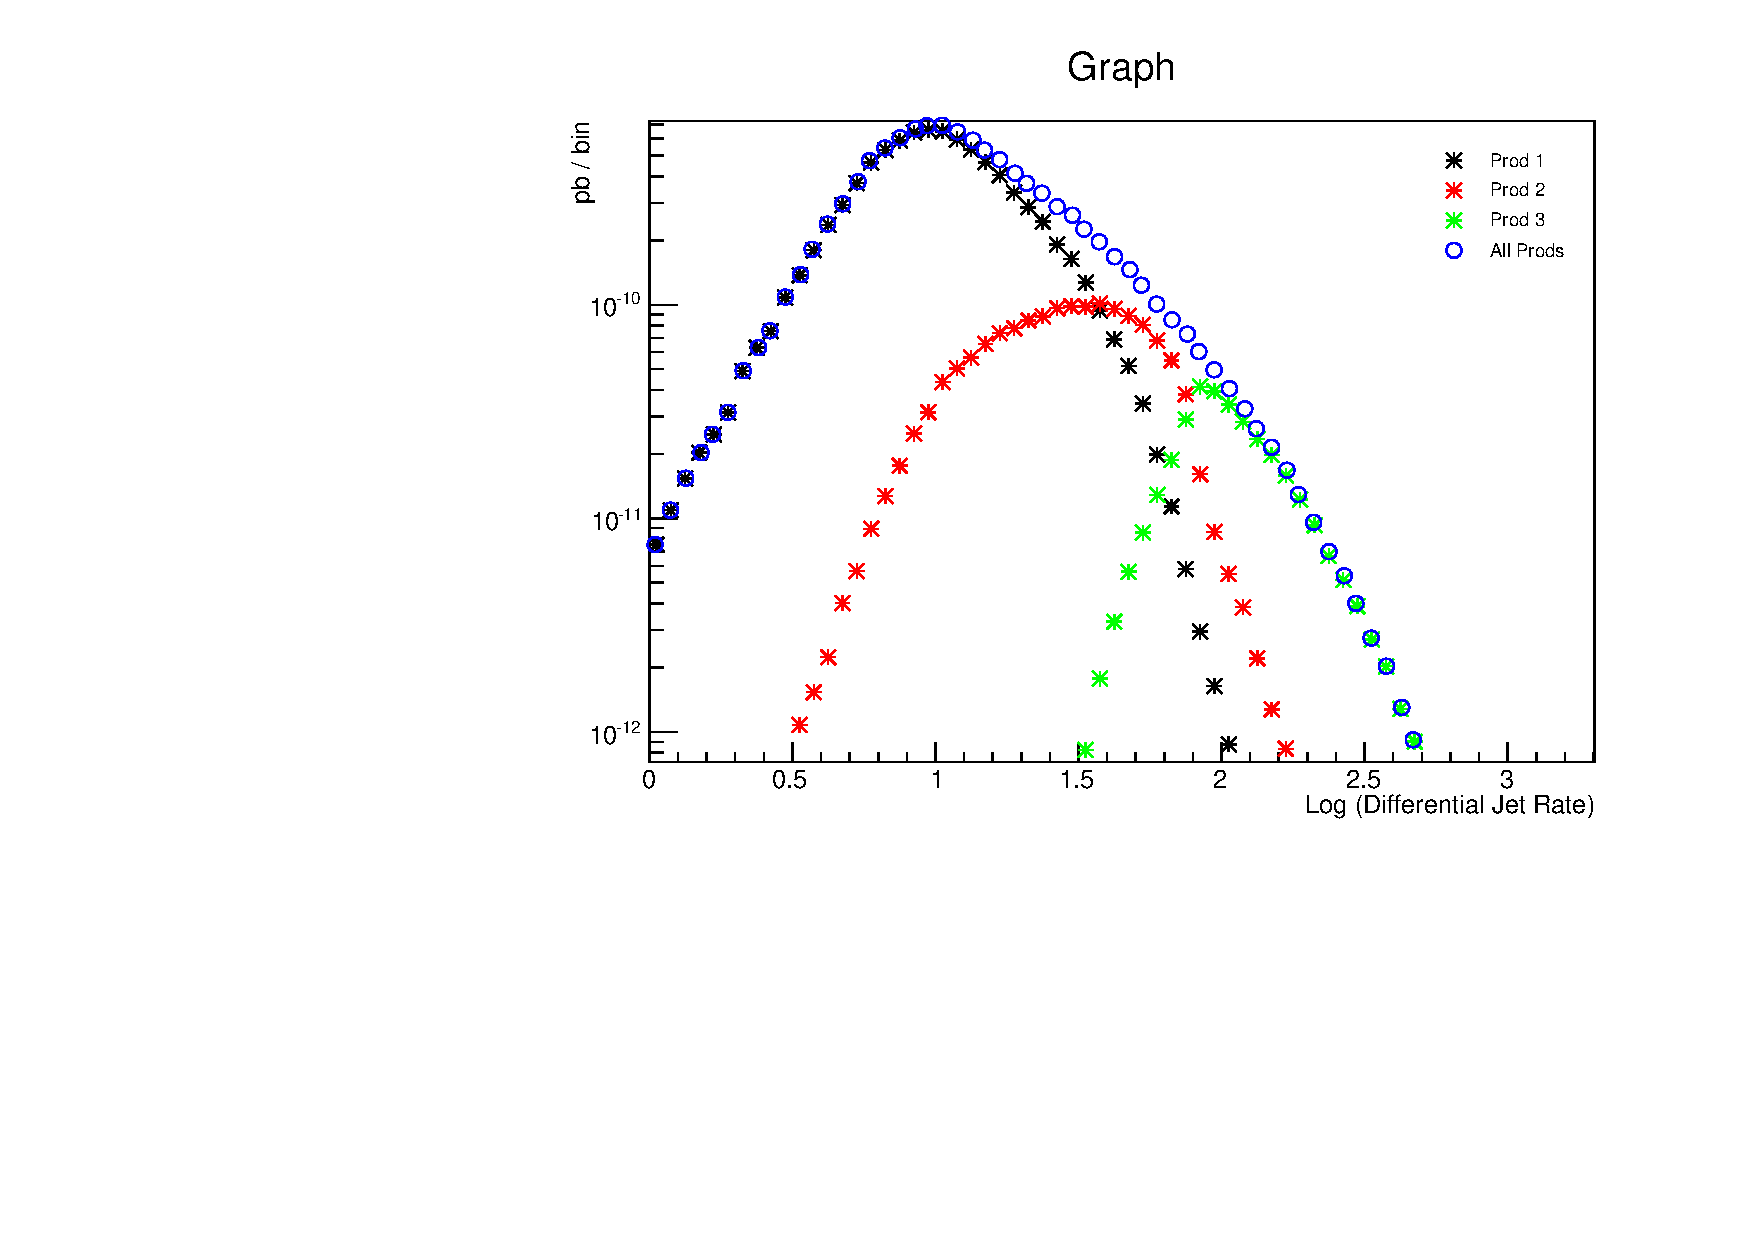
\includegraphics[width=0.45\linewidth]{figures/monojet_appendix/HistoJet2to3_80.pdf}
 	}
 	\hfill
 	\subfloat[$3\rightarrow4$ jets]{%
     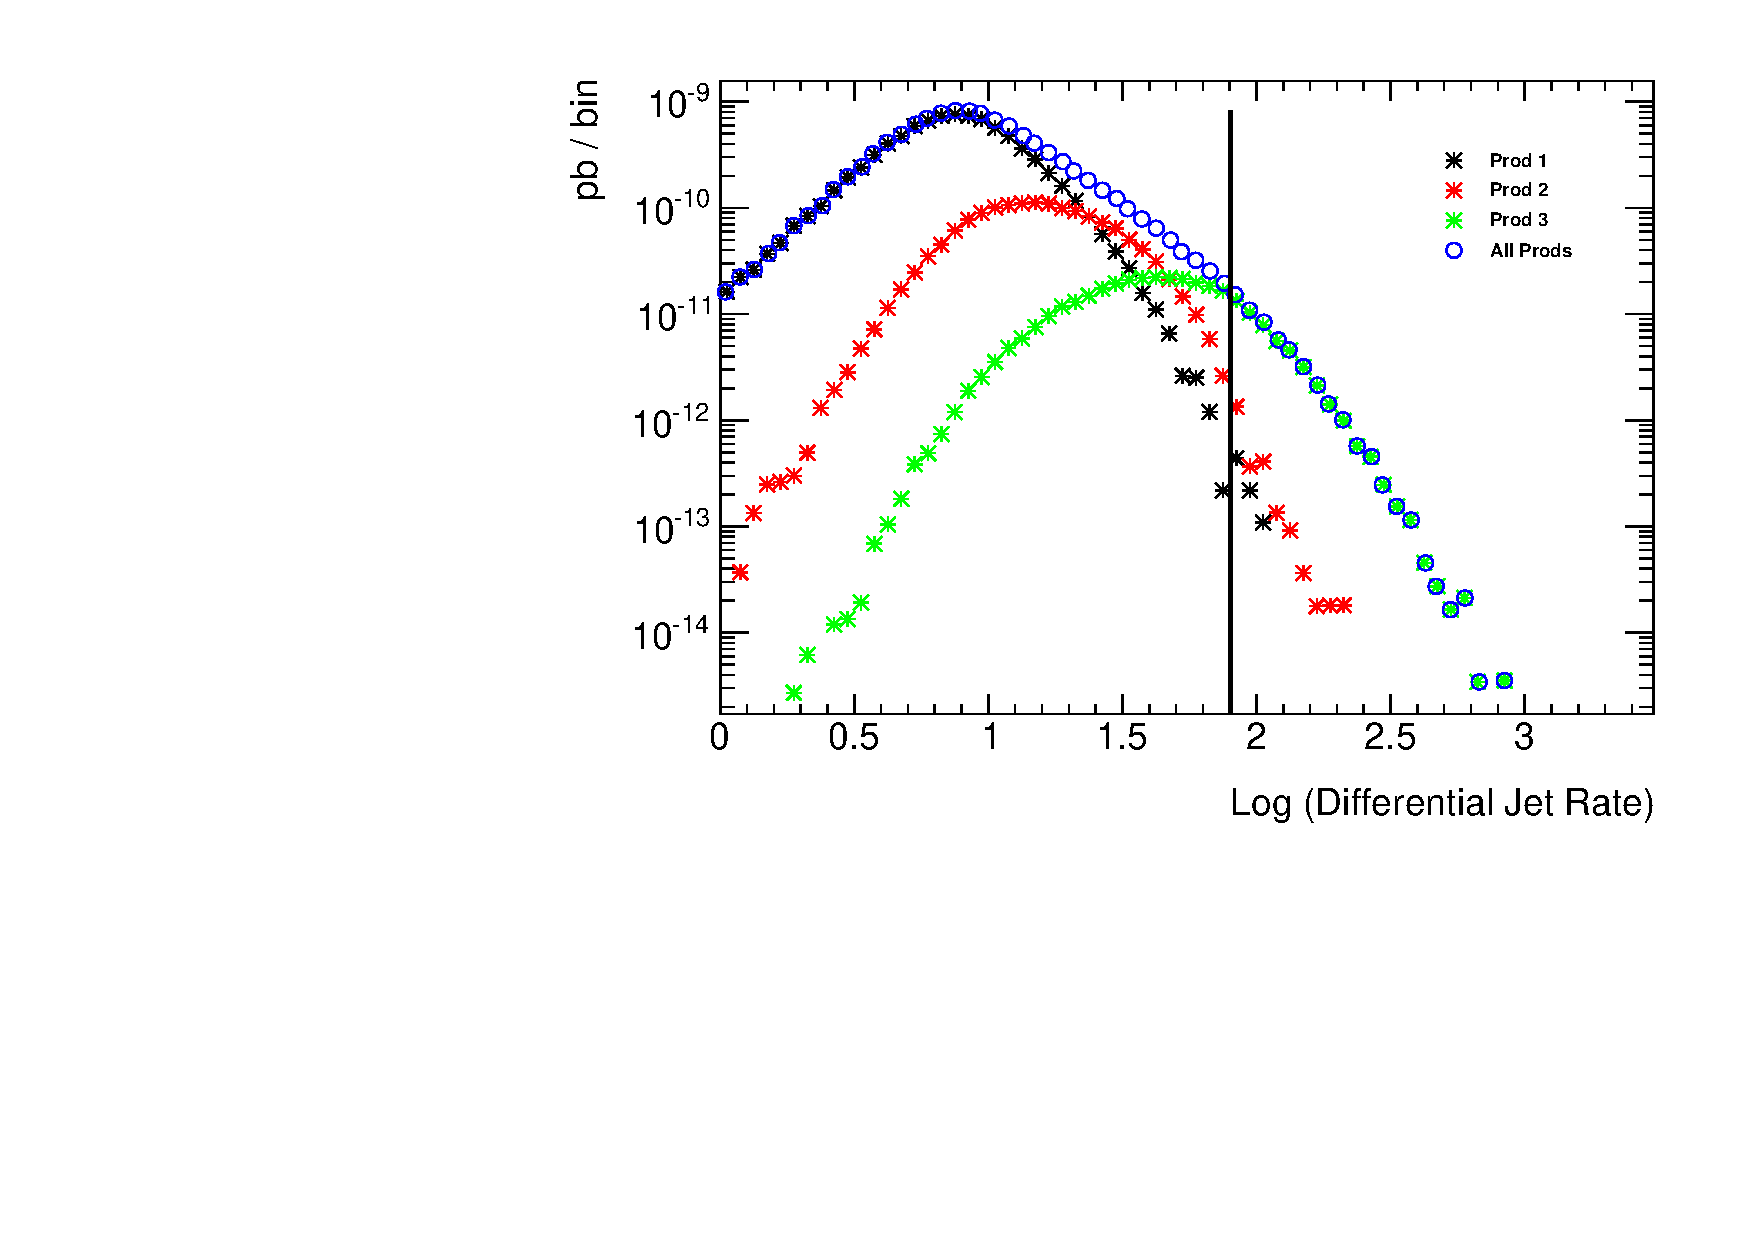
\includegraphics[width=0.45\linewidth]{figures/monojet_appendix/HistoJet3to4_80.pdf}
 	}
 	\hfill
 	\subfloat[$4\rightarrow5$ jets]{%
     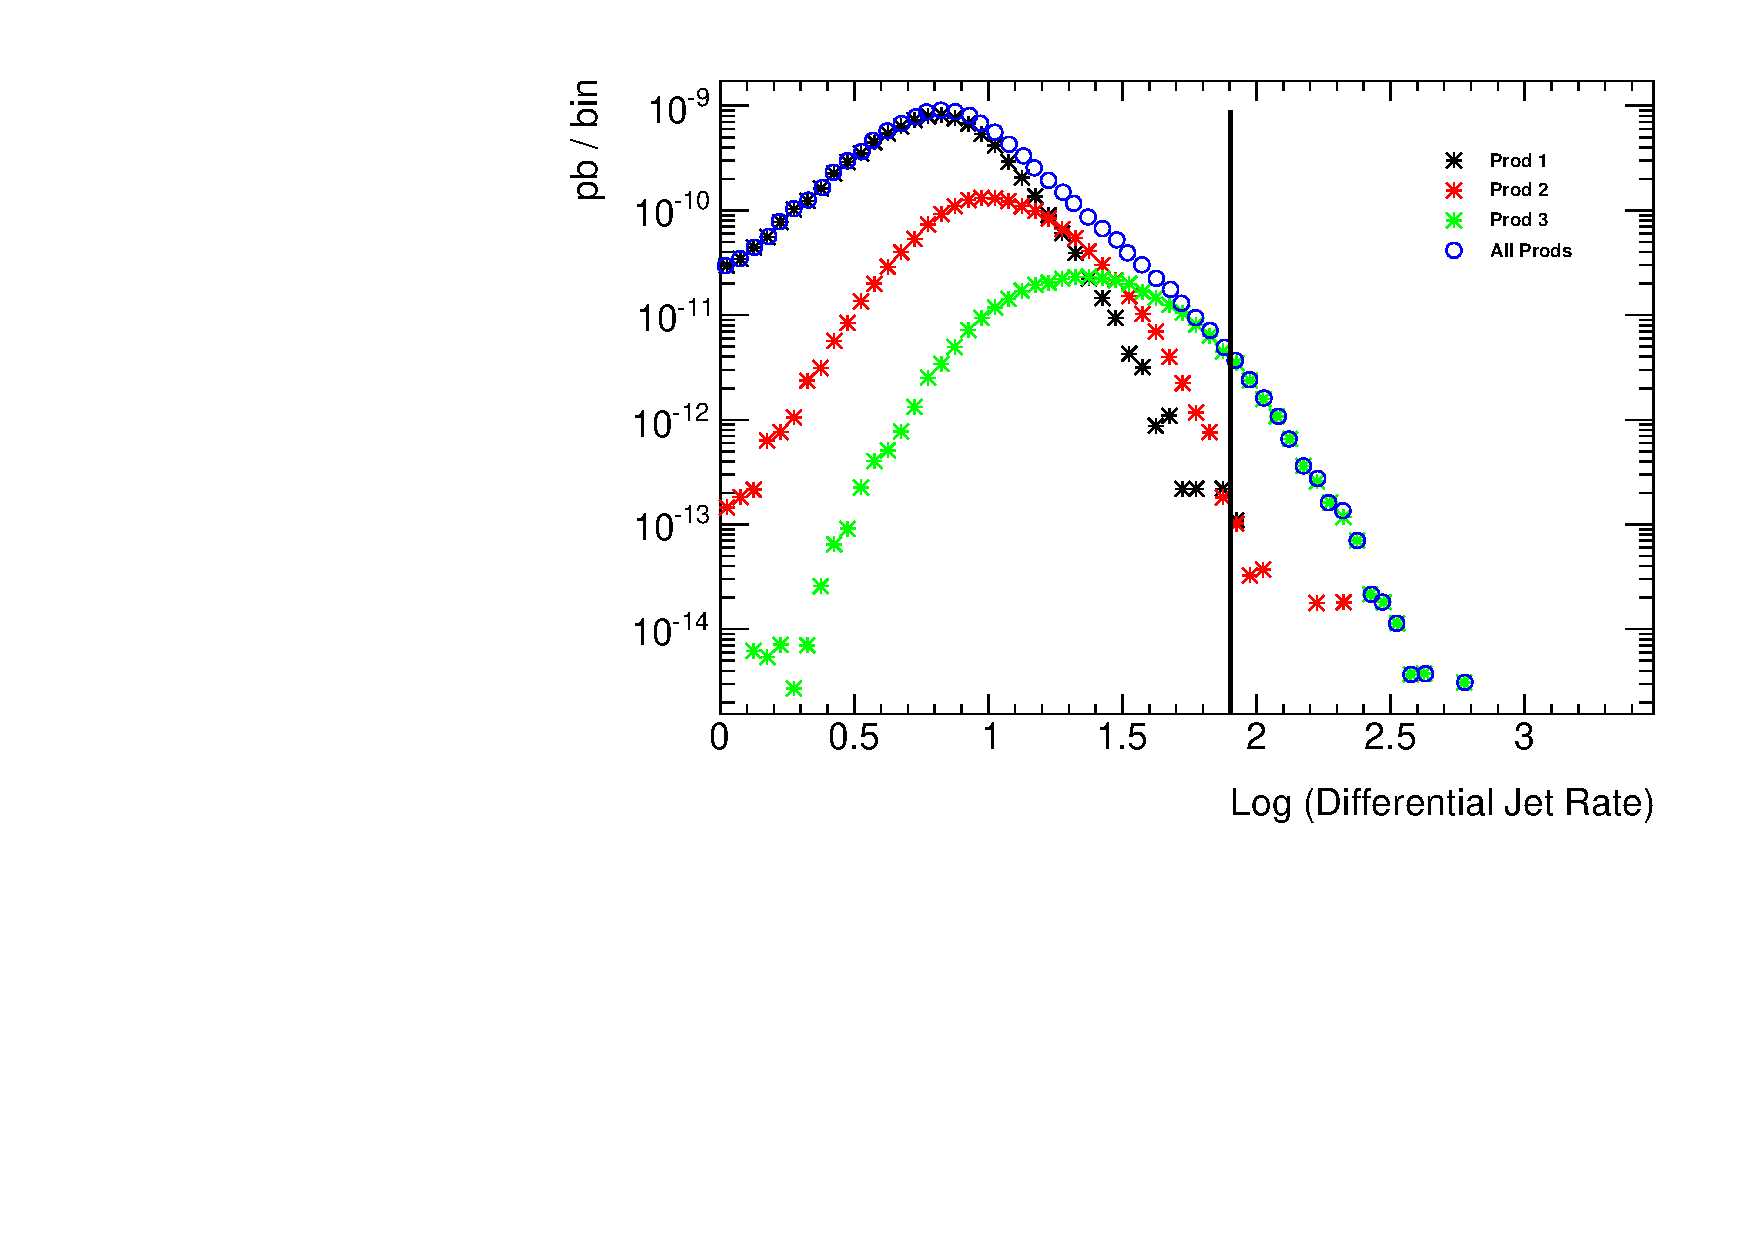
\includegraphics[width=0.45\linewidth]{figures/monojet_appendix/HistoJet4to5_80.pdf}
 	}
   \caption{Distributions of differential jet rates $\frac{dN_{i\to j}}{d \log_{10}(k_\textrm{cut})}$ for EFT D5 sample with CKKW-L matching scale at 80\,\gev. The 0-, 1- and 2-parton emission samples are generated separately and indicated in the plots as Prod 1, Prod 2 and Prod 3, respectively. A vertical line is drawn at the matching scale.}
   \label{fig:CKKW_D5_80}
 \end{figure}


 \begin{figure}[h!]
 	\centering  
 	\subfloat[$1\rightarrow2$ jets]{%
 		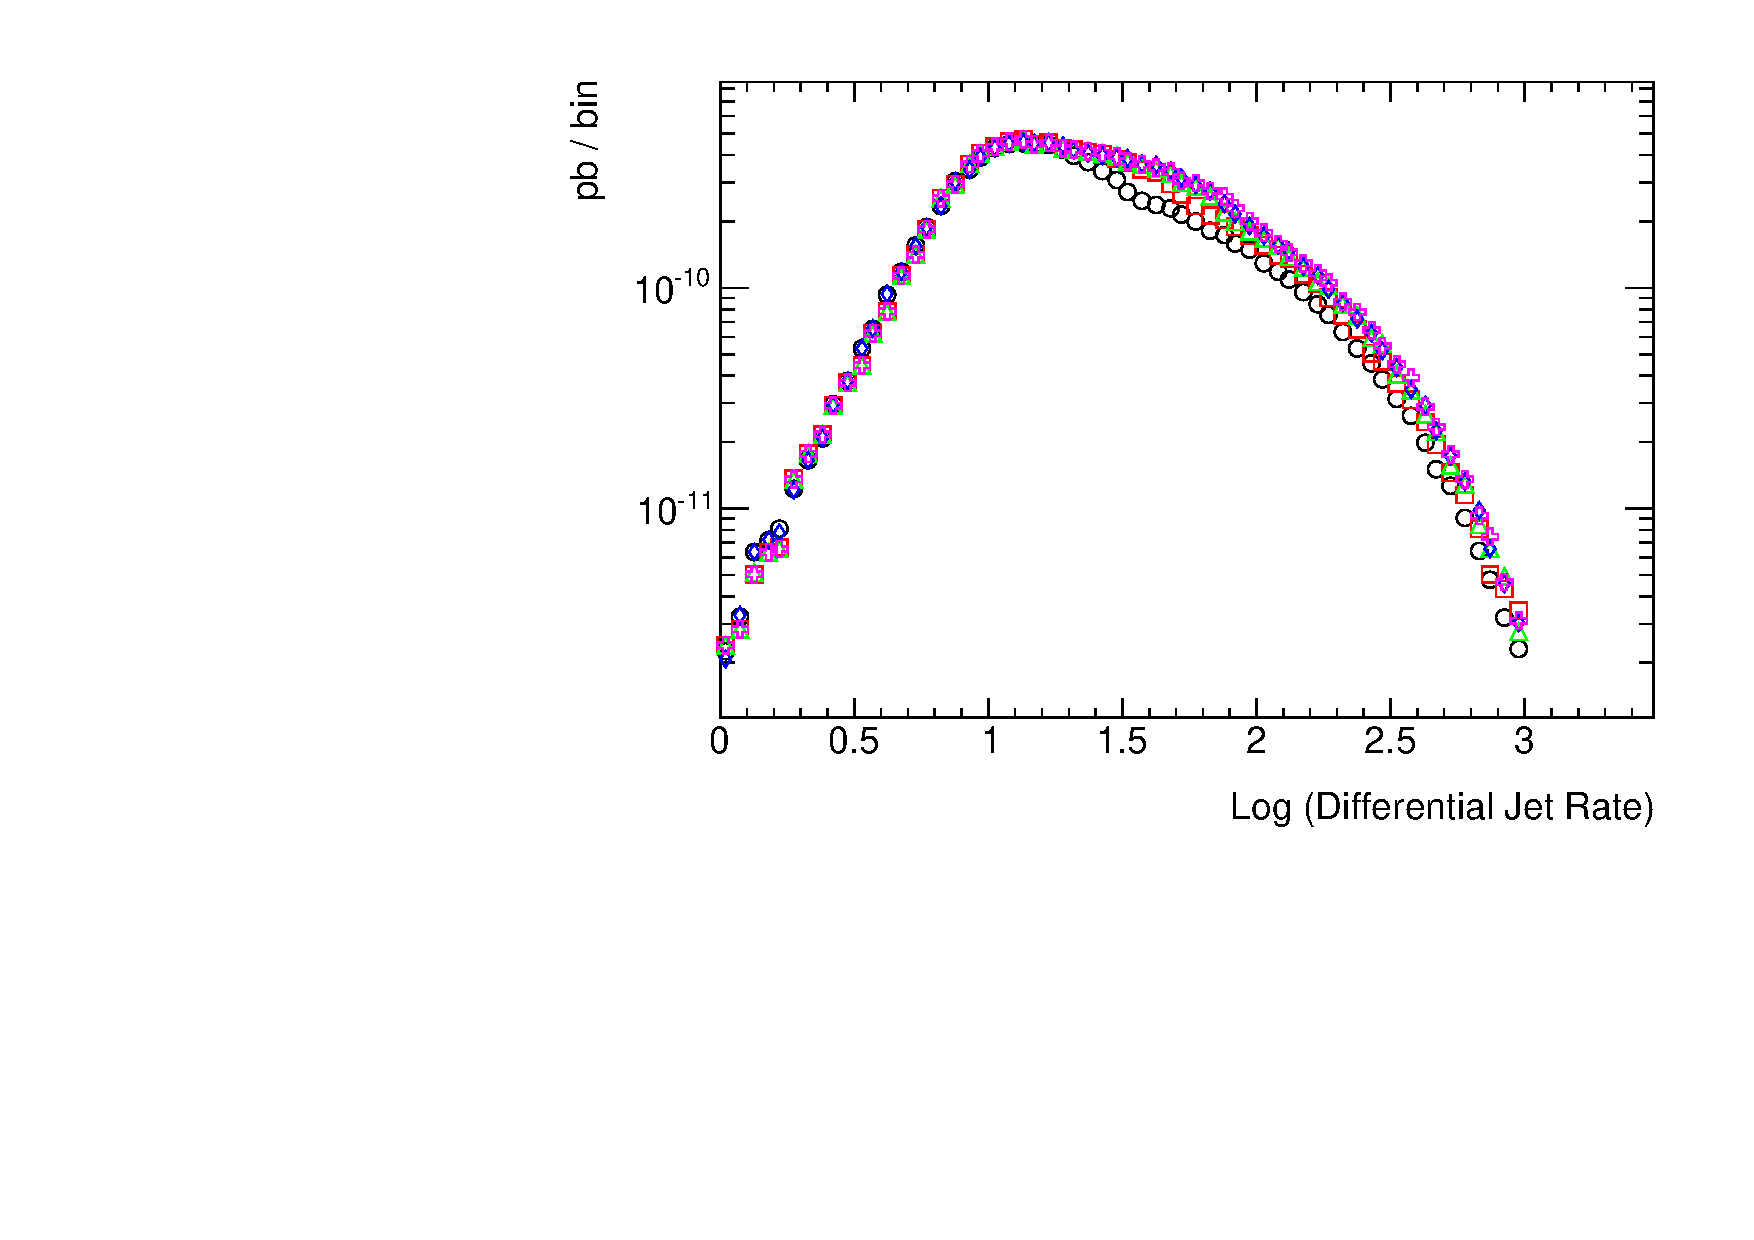
\includegraphics[width=0.45\linewidth]{figures/monojet_appendix/compare_plot_1.pdf}
 		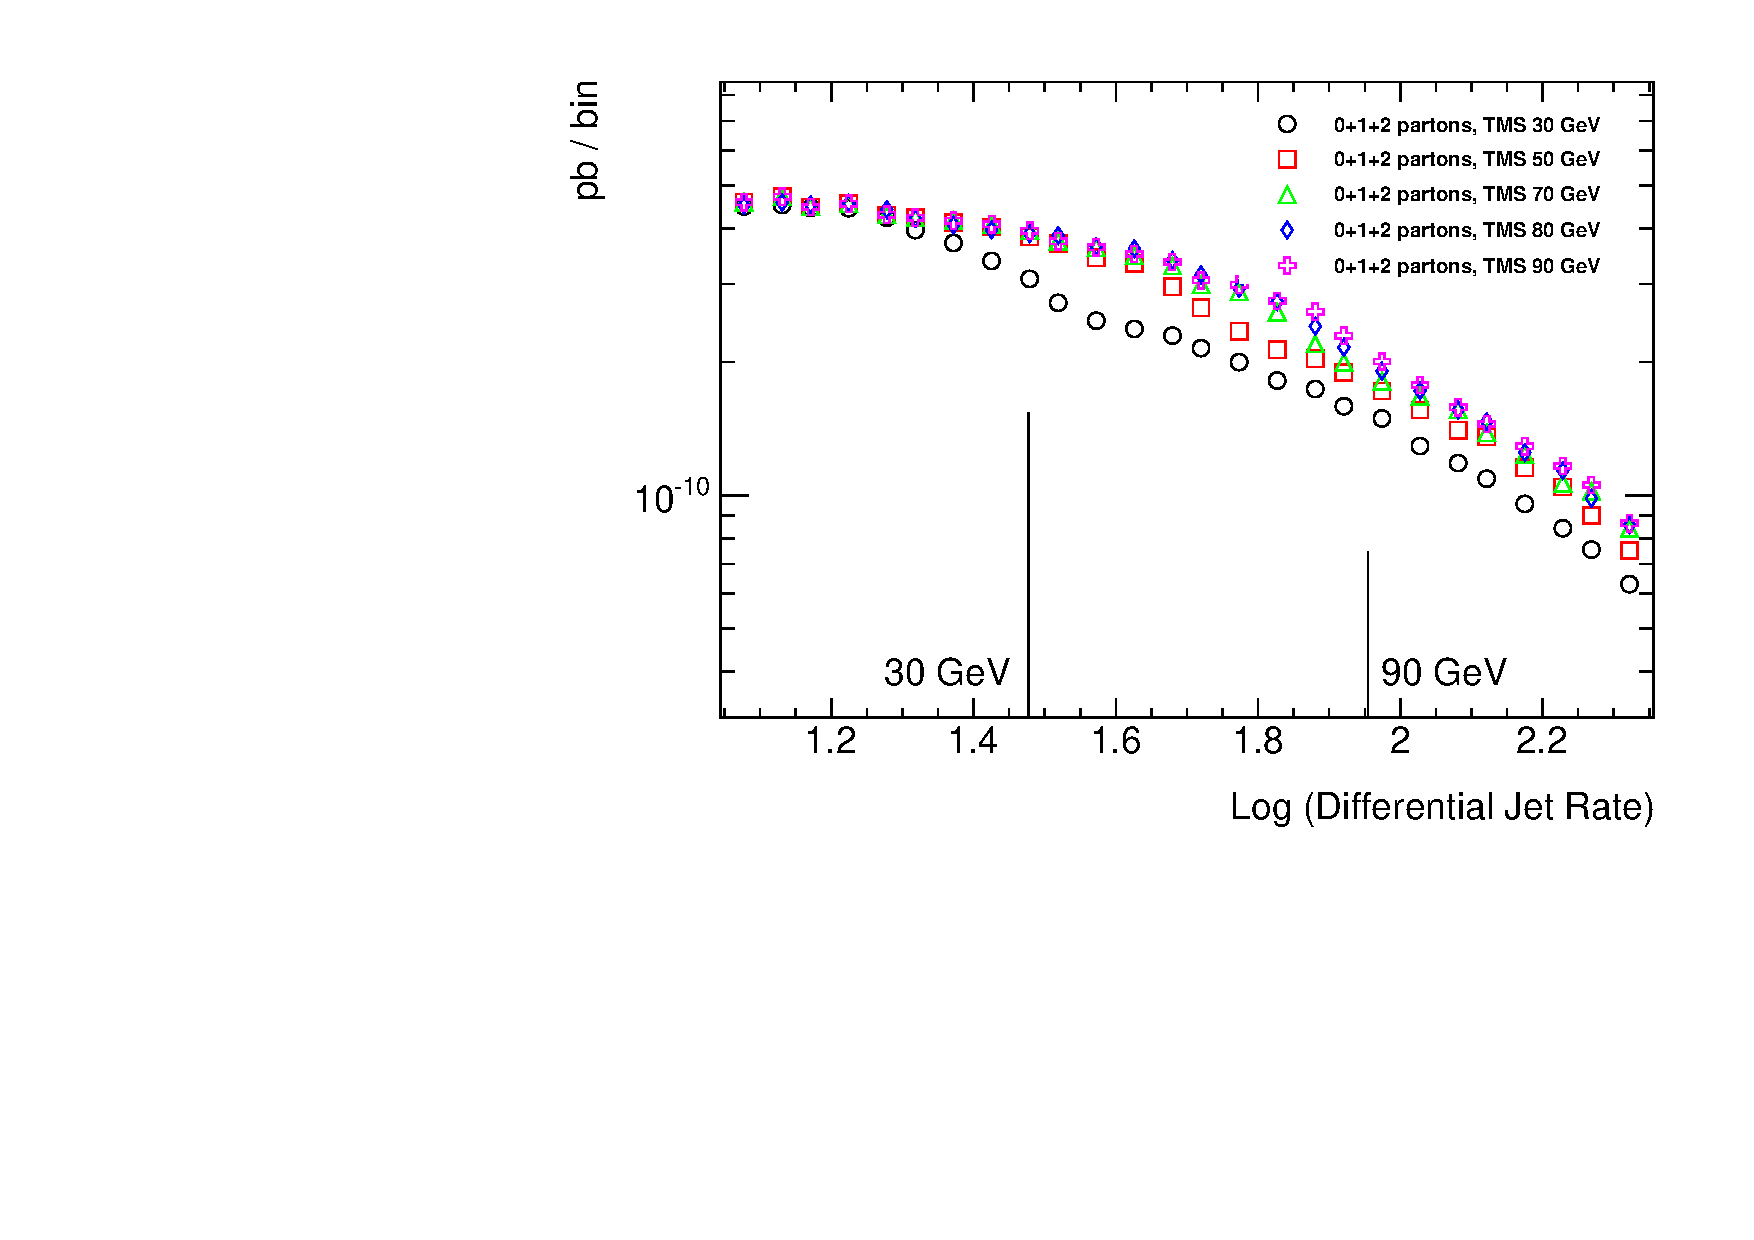
\includegraphics[width=0.45\linewidth]{figures/monojet_appendix/window_plot_1.pdf}
 	}
 	\hfill
 	\subfloat[$2\rightarrow3$ jets]{%
 		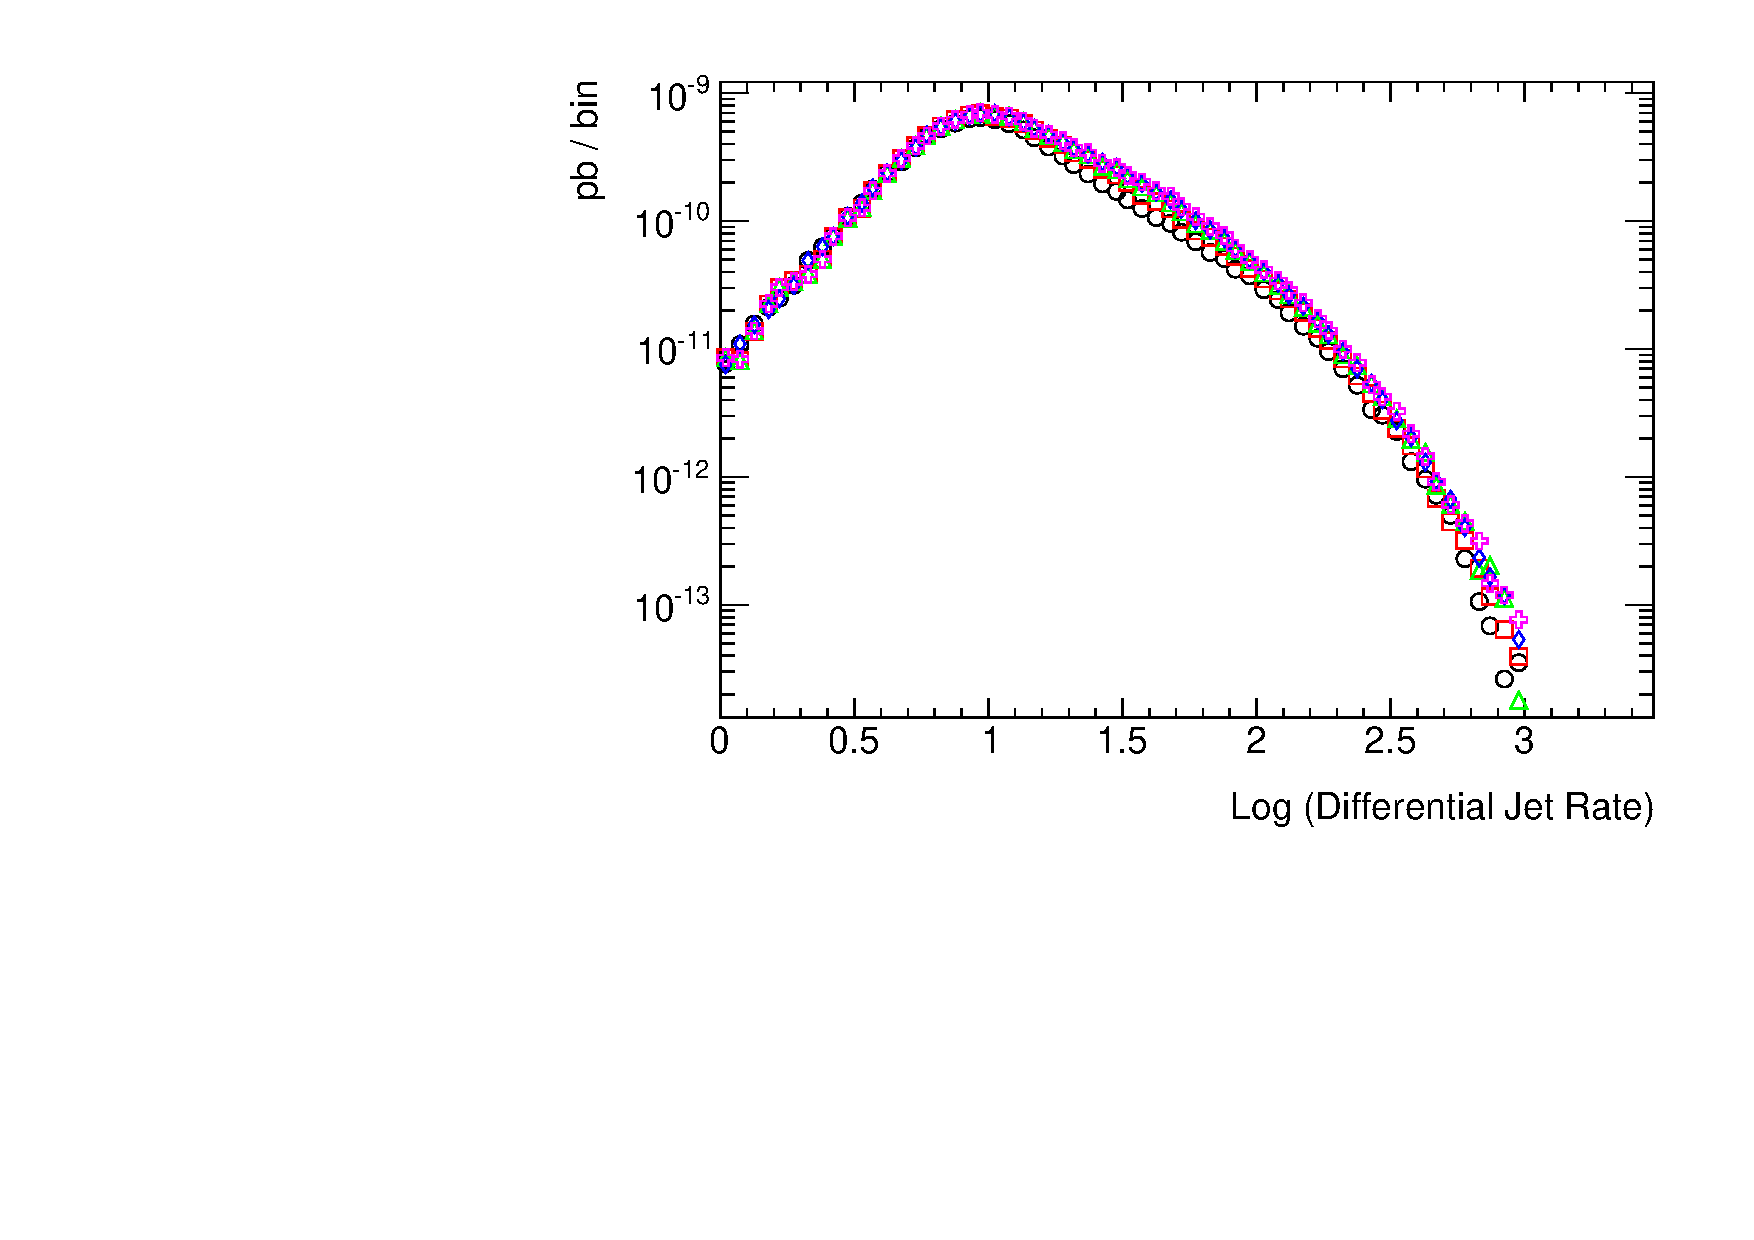
\includegraphics[width=0.45\linewidth]{figures/monojet_appendix/compare_plot_2.pdf}
 		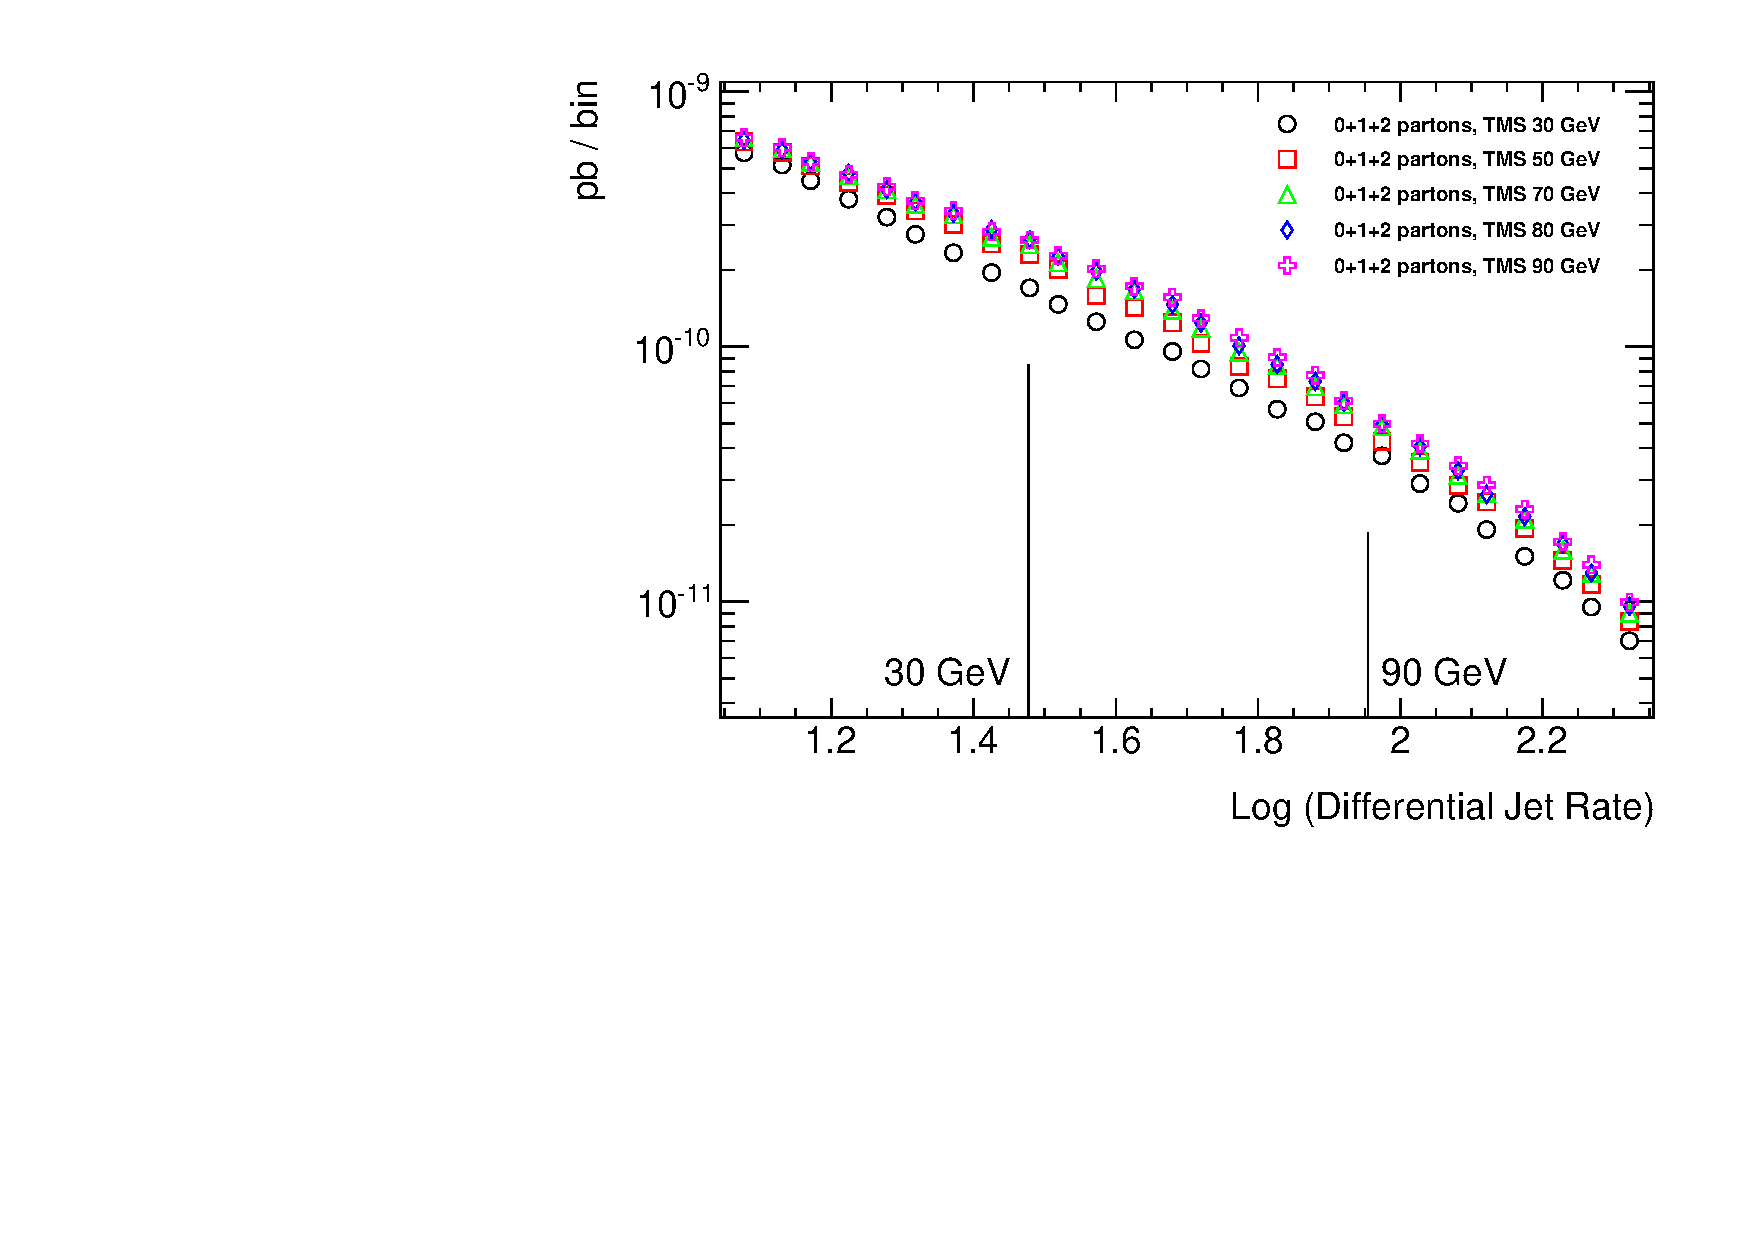
\includegraphics[width=0.45\linewidth]{figures/monojet_appendix/window_plot_2.pdf}
 	}
 	\hfill
 	\subfloat[$3\rightarrow4$ jets]{%
 		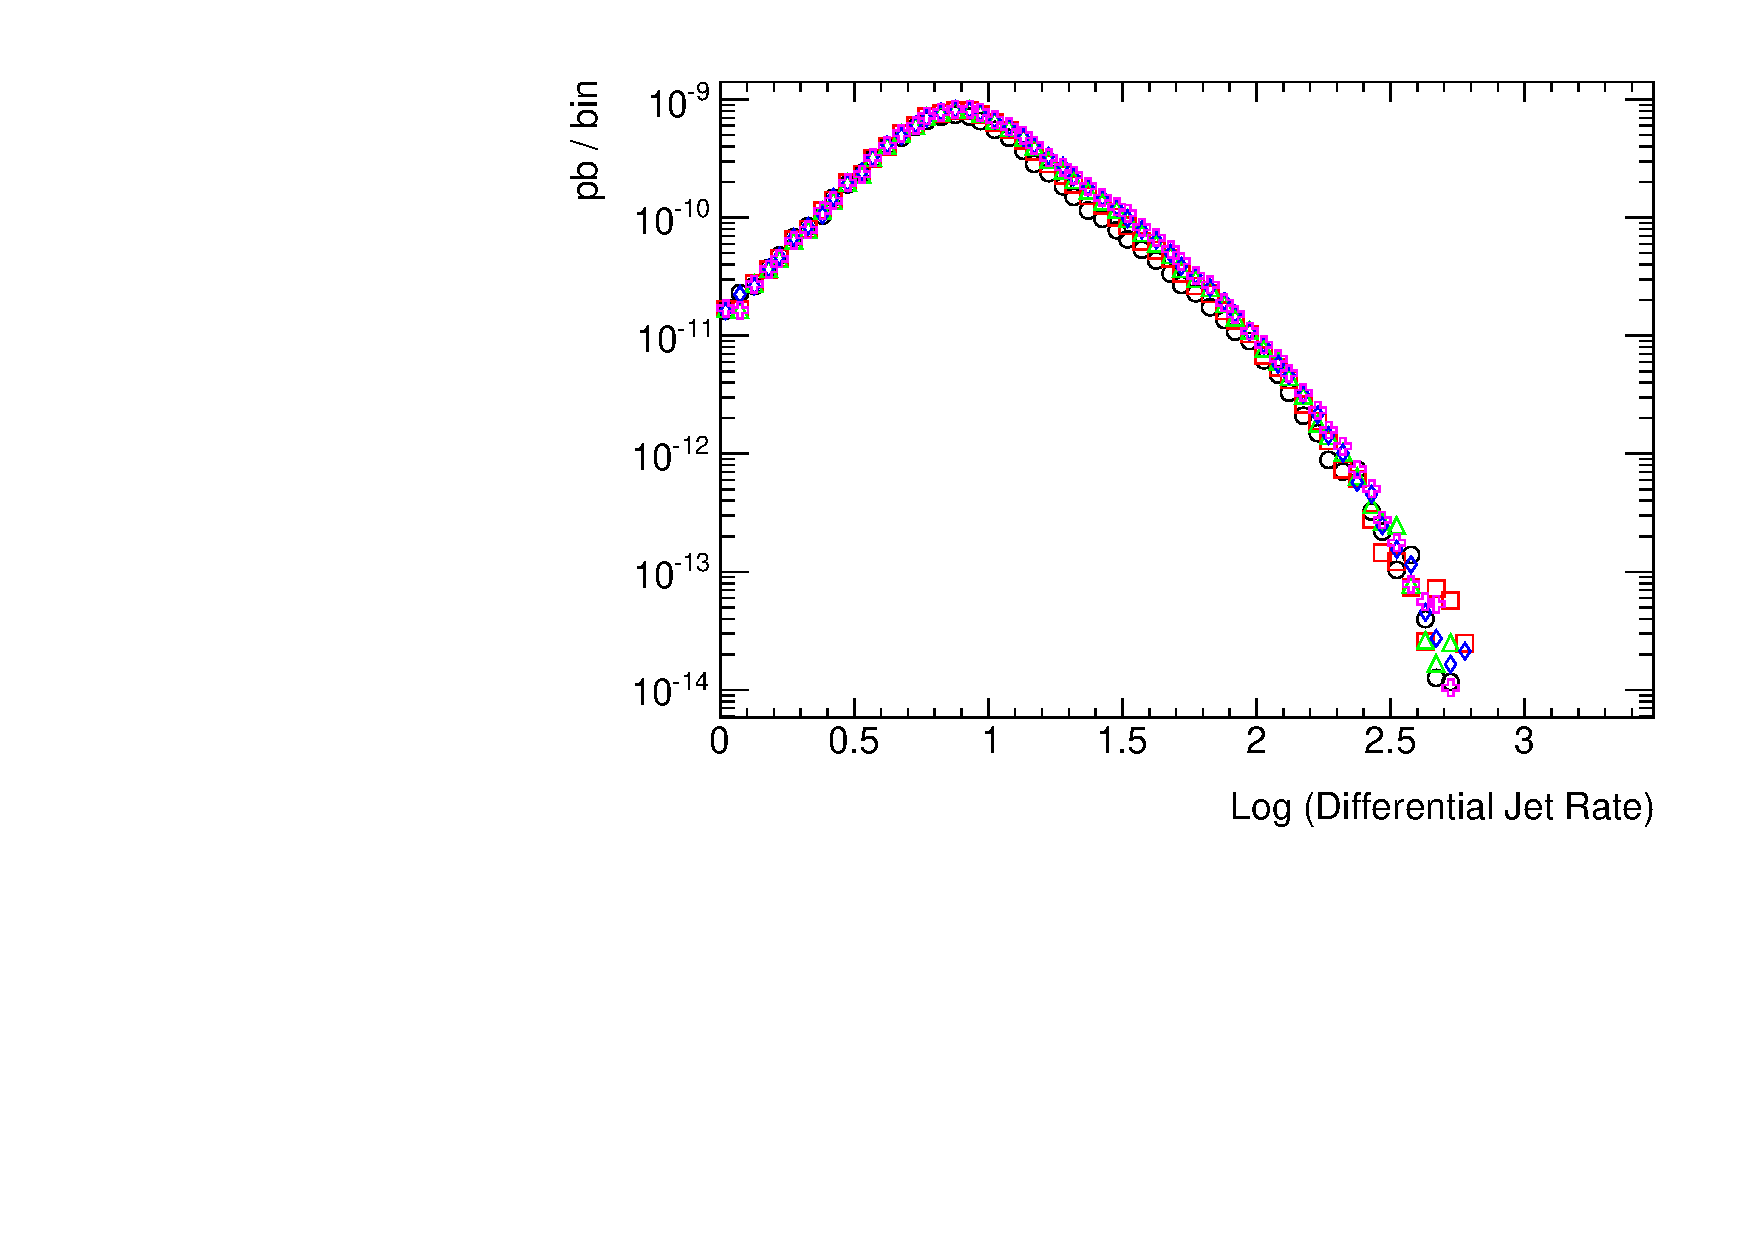
\includegraphics[width=0.45\linewidth]{figures/monojet_appendix/compare_plot_3.pdf}
 		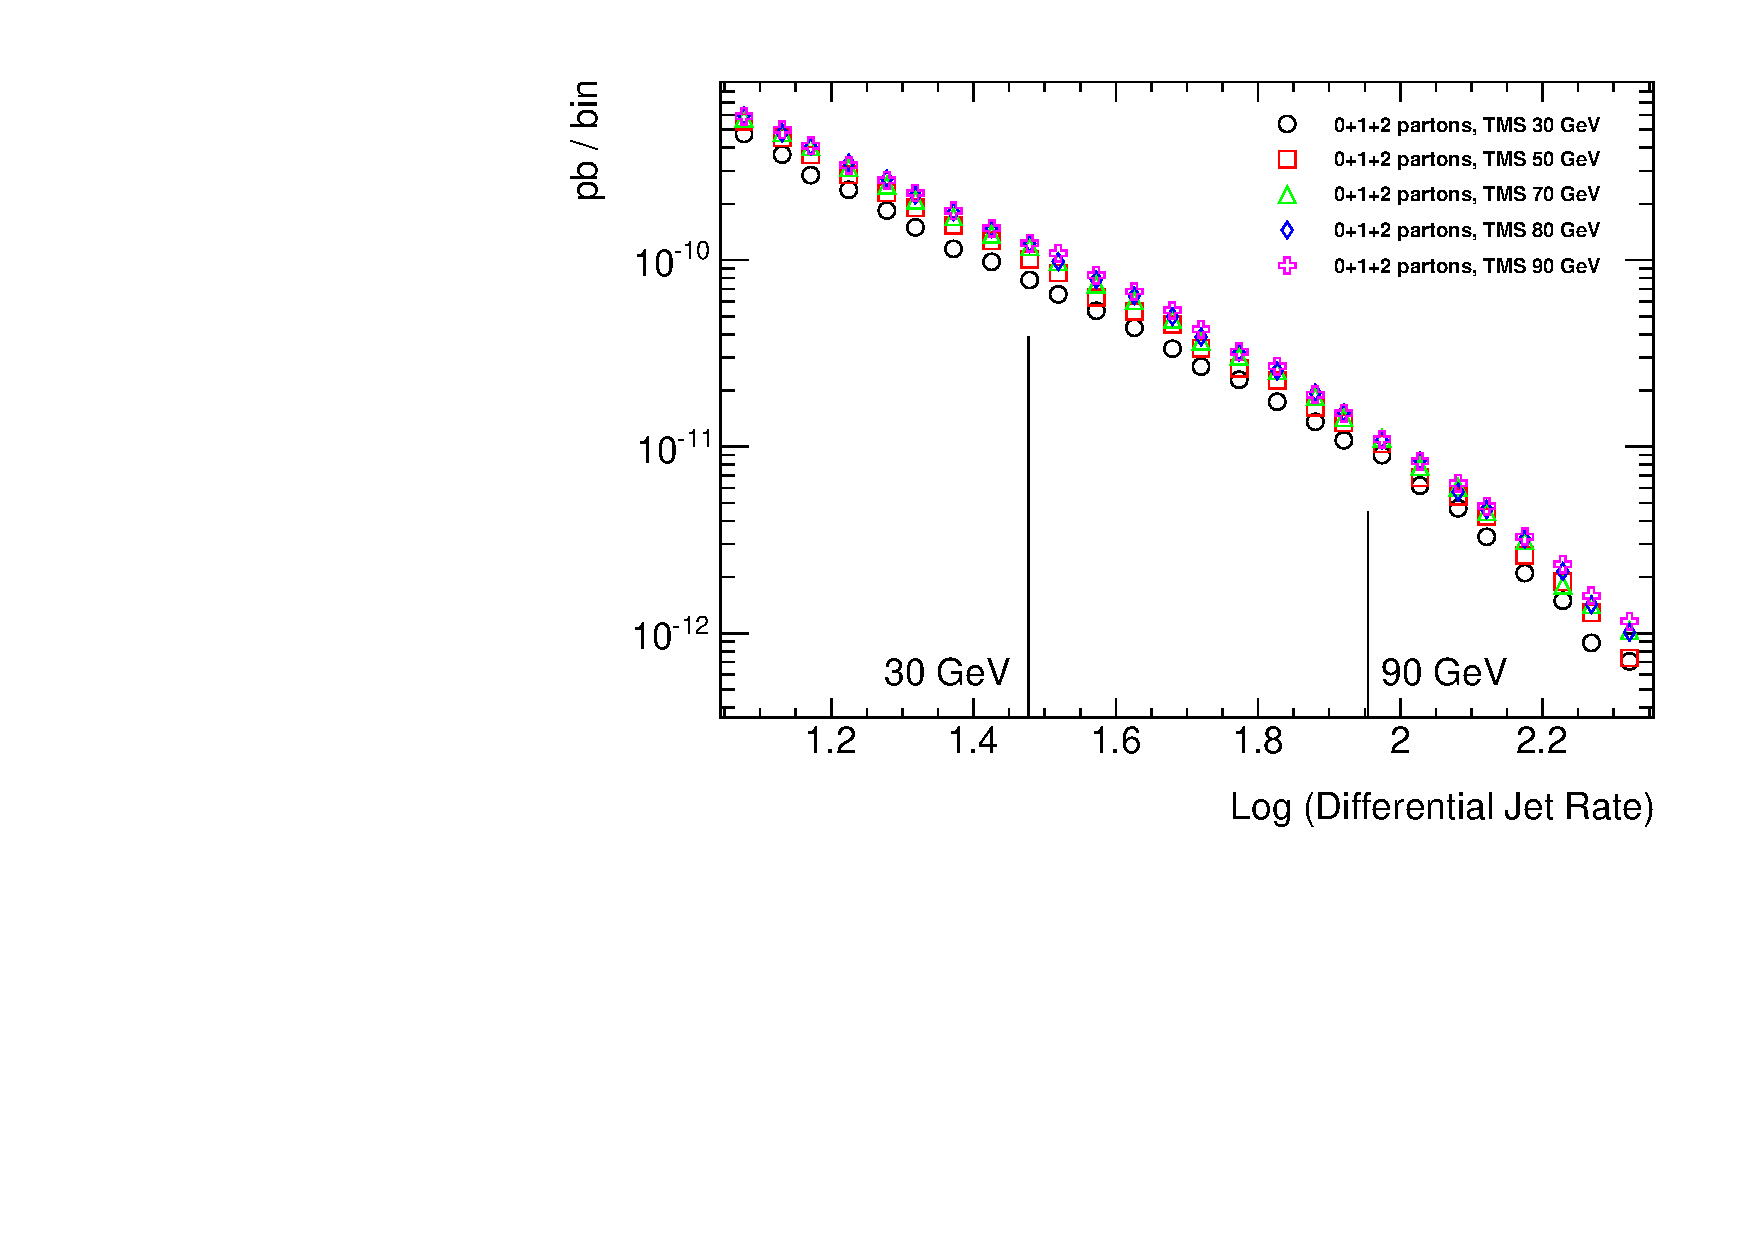
\includegraphics[width=0.45\linewidth]{figures/monojet_appendix/window_plot_3.pdf}
 	}
 	\hfill
 	\subfloat[$4\rightarrow5$ jets]{%
 		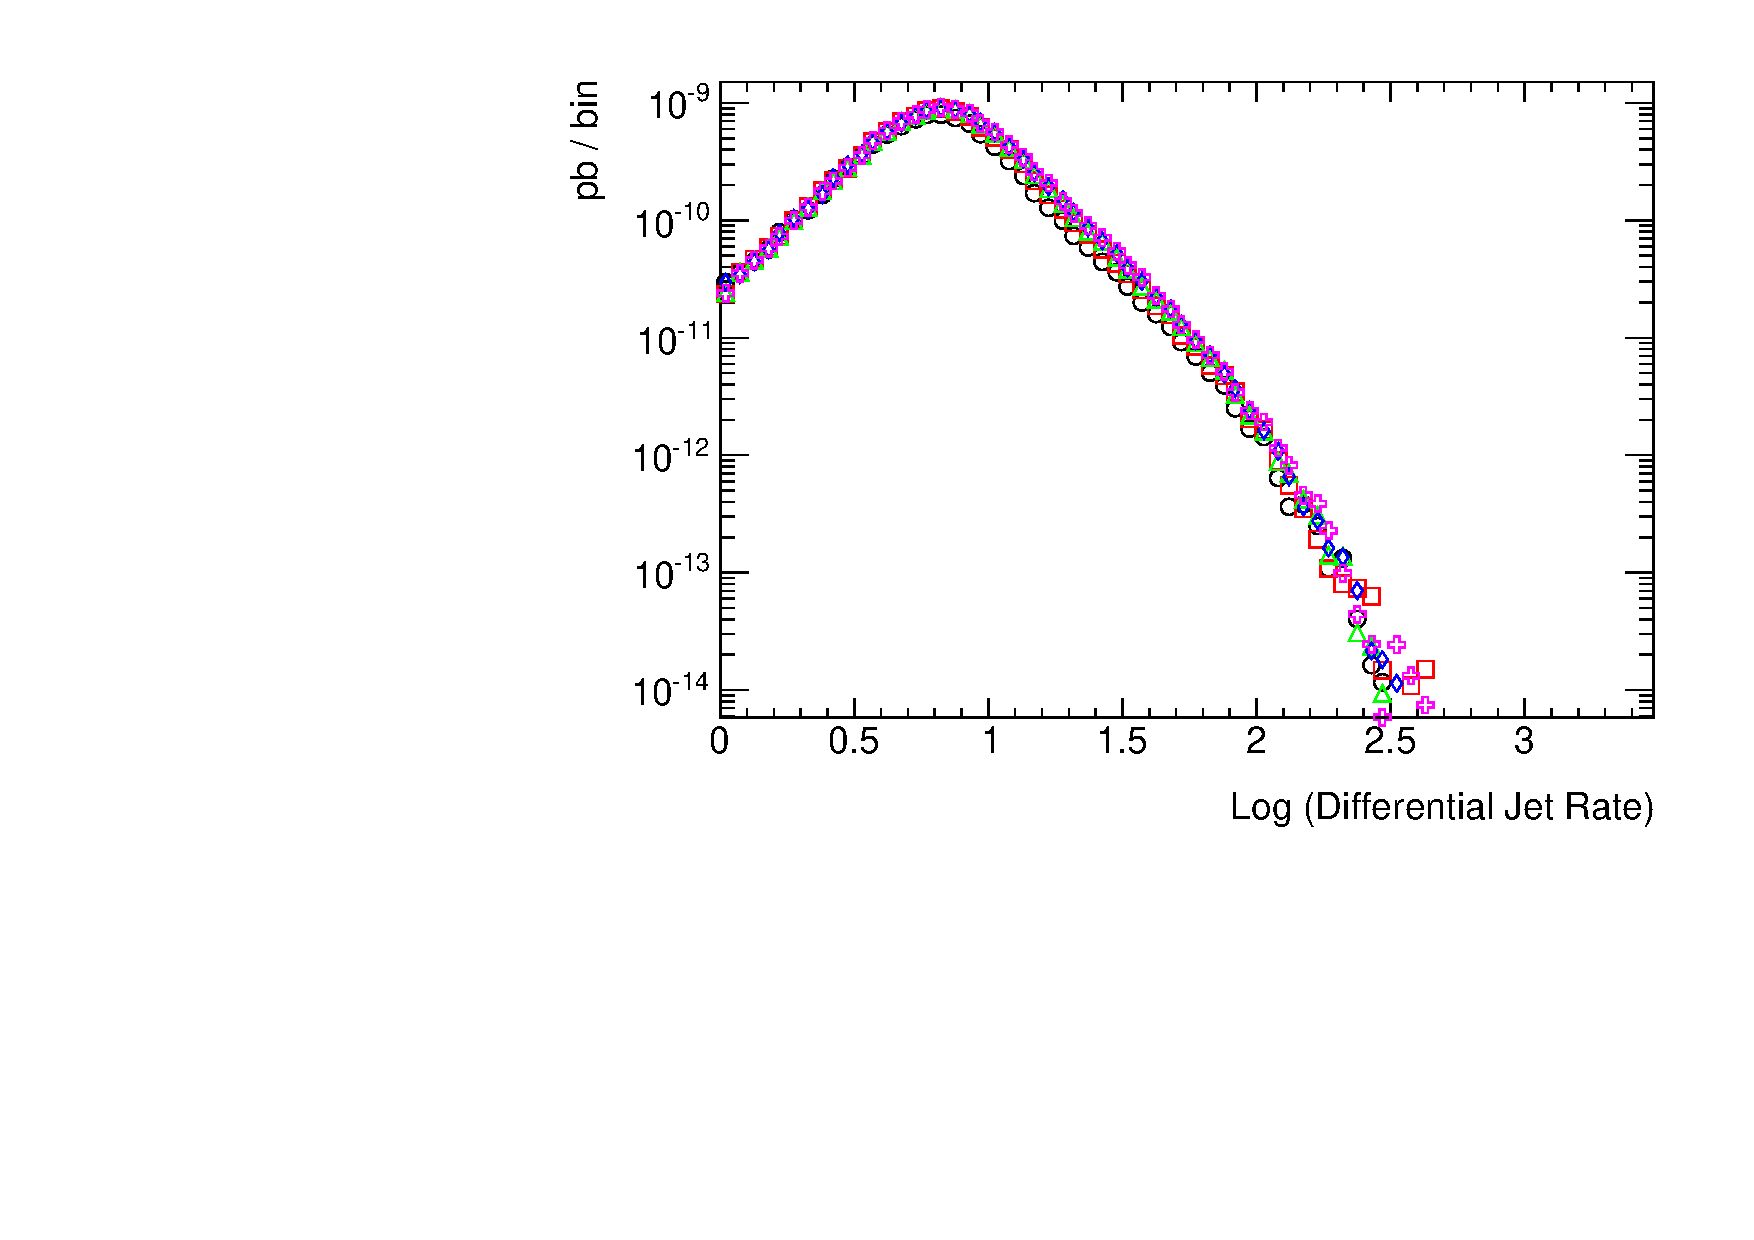
\includegraphics[width=0.45\linewidth]{figures/monojet_appendix/compare_plot_4.pdf}
 		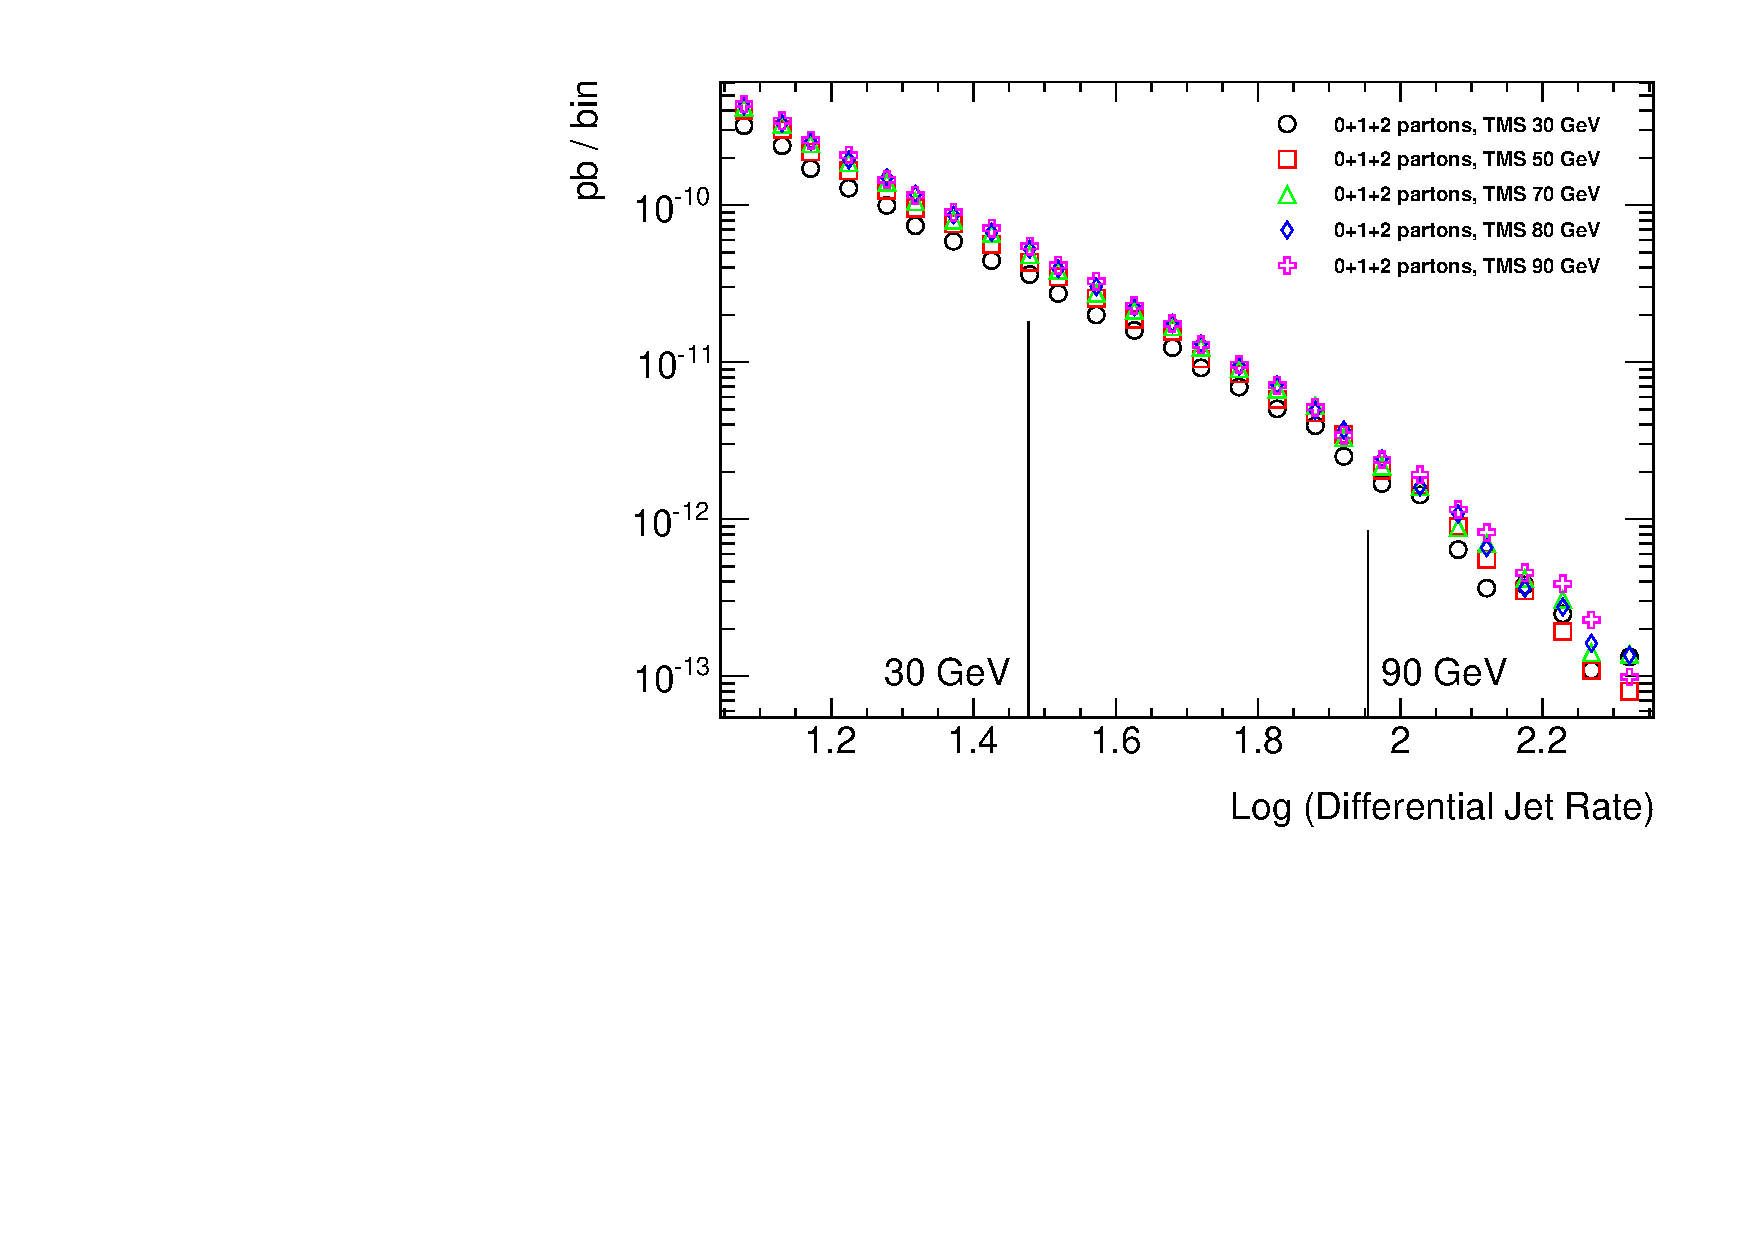
\includegraphics[width=0.45\linewidth]{figures/monojet_appendix/window_plot_4.pdf}
 	}
   \caption{Distributions of differential jet rates $\frac{dN_{i\to j}}{d \log_{10}(k_\textrm{cut})}$ for EFT D5 sample with CKKW-L matching scale at 30, 50, 70, 80 and 90\,\gev. A zoom of the region around the matching scale values is shown on right.}
   \label{fig:CKKW_D5_zoom}
 \end{figure}


%% \subsubsection{Parton emission multiplicity}
%% \label{sec:monojet_parton_emission}

 The prescription for the event generation given in Section\,\ref{sec:match_implementation} starts with the emission of 0 partons and ends with maxim 2 partons in addition. Producing the samples separately allows to investigate the relative composition of the individual samples in various parts of the phase space. Figure\,\ref{fig:Kine_D5_80} shows the \MET distribution of the EFT D5 sample with the matching scale at 80\,\gev. The plot reveals that the 0-parton sample gives the dominant contribution in the region below the matching scale value that rapidly decreases at higher \MET. Assuming the lowest analysis \MET cut in Run-2 mono-jet analyses at 300\,\gev, the generation of the 0-parton emission sample can be safely omitted as it only gives $<1\%$ contribution at $\MET>300\,\gev$. For the 1- and 2-parton emission samples, one can use a generator cut on the leading parton $\pT$, \texttt{ptj1min}, in order to avoid generating low \MET events that are irrelevant for the analysis.

 \begin{figure}[h!]
 	\centering  
 %	\subfloat[Missing transverse momentum]{%
     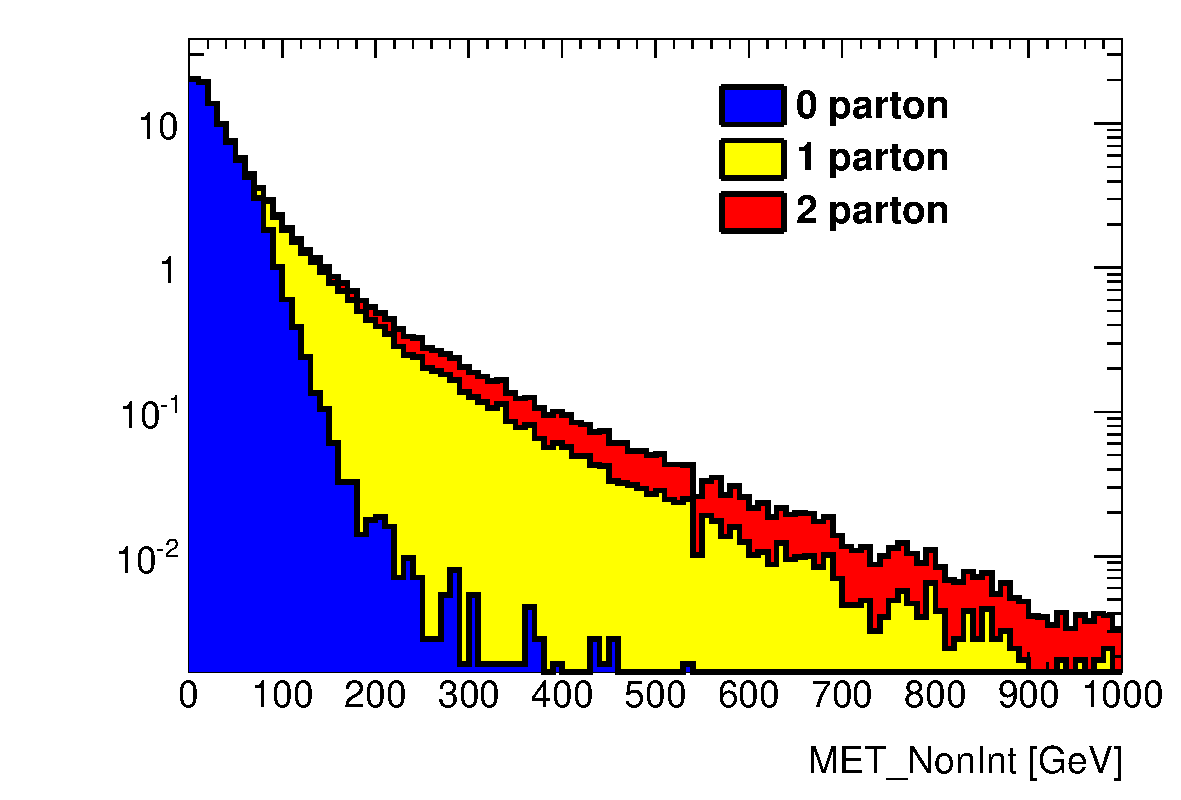
\includegraphics[width=0.95\linewidth]{figures/monojet_appendix/MET_matching80.pdf}
 %	}
 %	\hfill
 %	\subfloat[Transverse momentum of leading jet]{%
 %    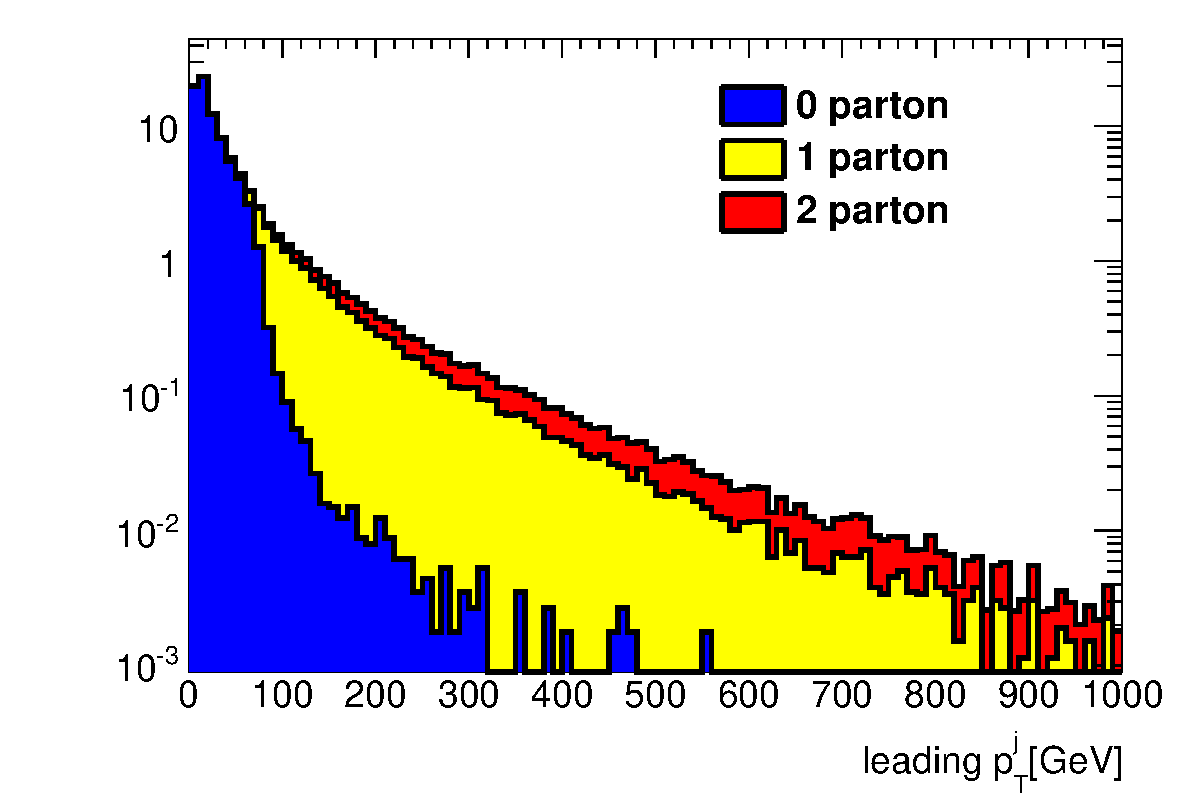
\includegraphics[width=0.95\linewidth]{figures/monojet_appendix/jet1pt_matching80.pdf}
 %	}
 %	\hfill
 %	\subfloat[Transverse momentum of subleading jet]{%
 %    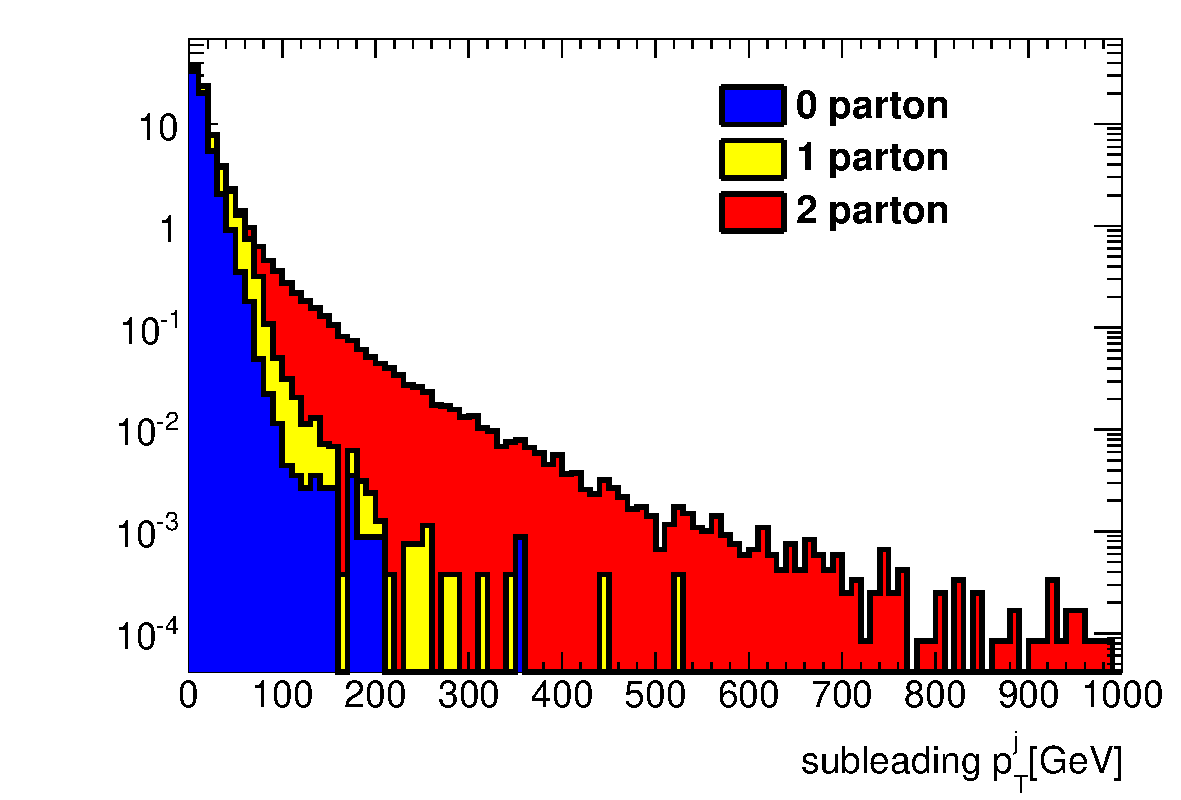
\includegraphics[width=0.95\linewidth]{figures/monojet_appendix/jet2pt_matching80.pdf}
 %	}
 %	\caption{Kinematics distributions for EFT D5 sample with CKKW matching scale at 80 \gev. 0-, 1- and 2-parton emission cases are generated separately and added together by cross sections. The 0-parton emission case has very limited contribution for missing transverse energy larger than 300 \gev region.}
 	\caption{Missing transverse momentum distributions for EFT D5 sample with CKKW-L matching scale at 80\,\gev. Individual contributions from the 0-, 1- and 2-parton emission samples are shown.}
 	\label{fig:Kine_D5_80}
 \end{figure}



In order to describe the signal kinematics correctly and save time during MC production, the parton emissions will only be generated up to a certain multiplicity. The higher multiplicity samples usually have small enough cross sections and the corresponding parts of the phase space can be sufficiently approximated by parton showering in \pythiaEight.
A dedicated study comparing samples generated with up to 1-, 2-, or 3-parton multiplicities was performed, using again the settings for the CKKW-L $k_T$-merging with the 80\,\gev matching scale and the \texttt{Merging:nJetMax} parameter adjusted accordingly.
Figure\,\ref{fig:RatioKine_D5} shows the \MET distribution of the samples at $\MET>250\,\gev$.

%While there is a $\sim10\%$ difference observed between the samples with up to 1 parton and up to 3 partons at low $\MET$, only marginal difference is seen between the samples generated with up to 2 and 3 partons.

With an event selection requiring \MET and the leading jet \pT being larger than $250\,\gev$ and allowing for up to 3 jets with $\pT>30\,\gev$, the sample generated with up to 1 parton has 17.4\% smaller yield compared to the sample with up to 3 partons, while the yield of the sample with up to 2 partons is only 2.2\% smaller.
Note the jet multiplicity cut is important here as the agreement between the two samples improves at higher \MET when the cut is not applied.
%At \MET>400\,\gev$, 0+1 parton emission has 16.8\% yield less and 0+1+2 parton emission has 2.4\% less compared to 0+1+2+3 parton emission. With $\MET>600\,\gev$, 0+1 parton emission has 16.5\% yield less and 0+1+2 parton emission has 2.9\% less compared to 0+1+2+3 parton emission. The same numbers hold if a symmetric cut is added on leading jet transverse momentum.
A similar comparison is shown in Fig.\,\ref{fig:RatioKine_D5_2} for the jet multiplicity in the events with the leadning jet $\pT>250\,\gev$, where an agreement at the level of $\sim3\%$ between the samples with up to 2 and 3 parton emissions is observed for number of jets up to 7.
This justifies it is sufficient to produce samples with up to 2 parton emissions only at the generator level and ignore generating higher parton emissions.


\begin{figure}[h!]
	\centering  
	\subfloat[No jet multiplicity cut]{%
		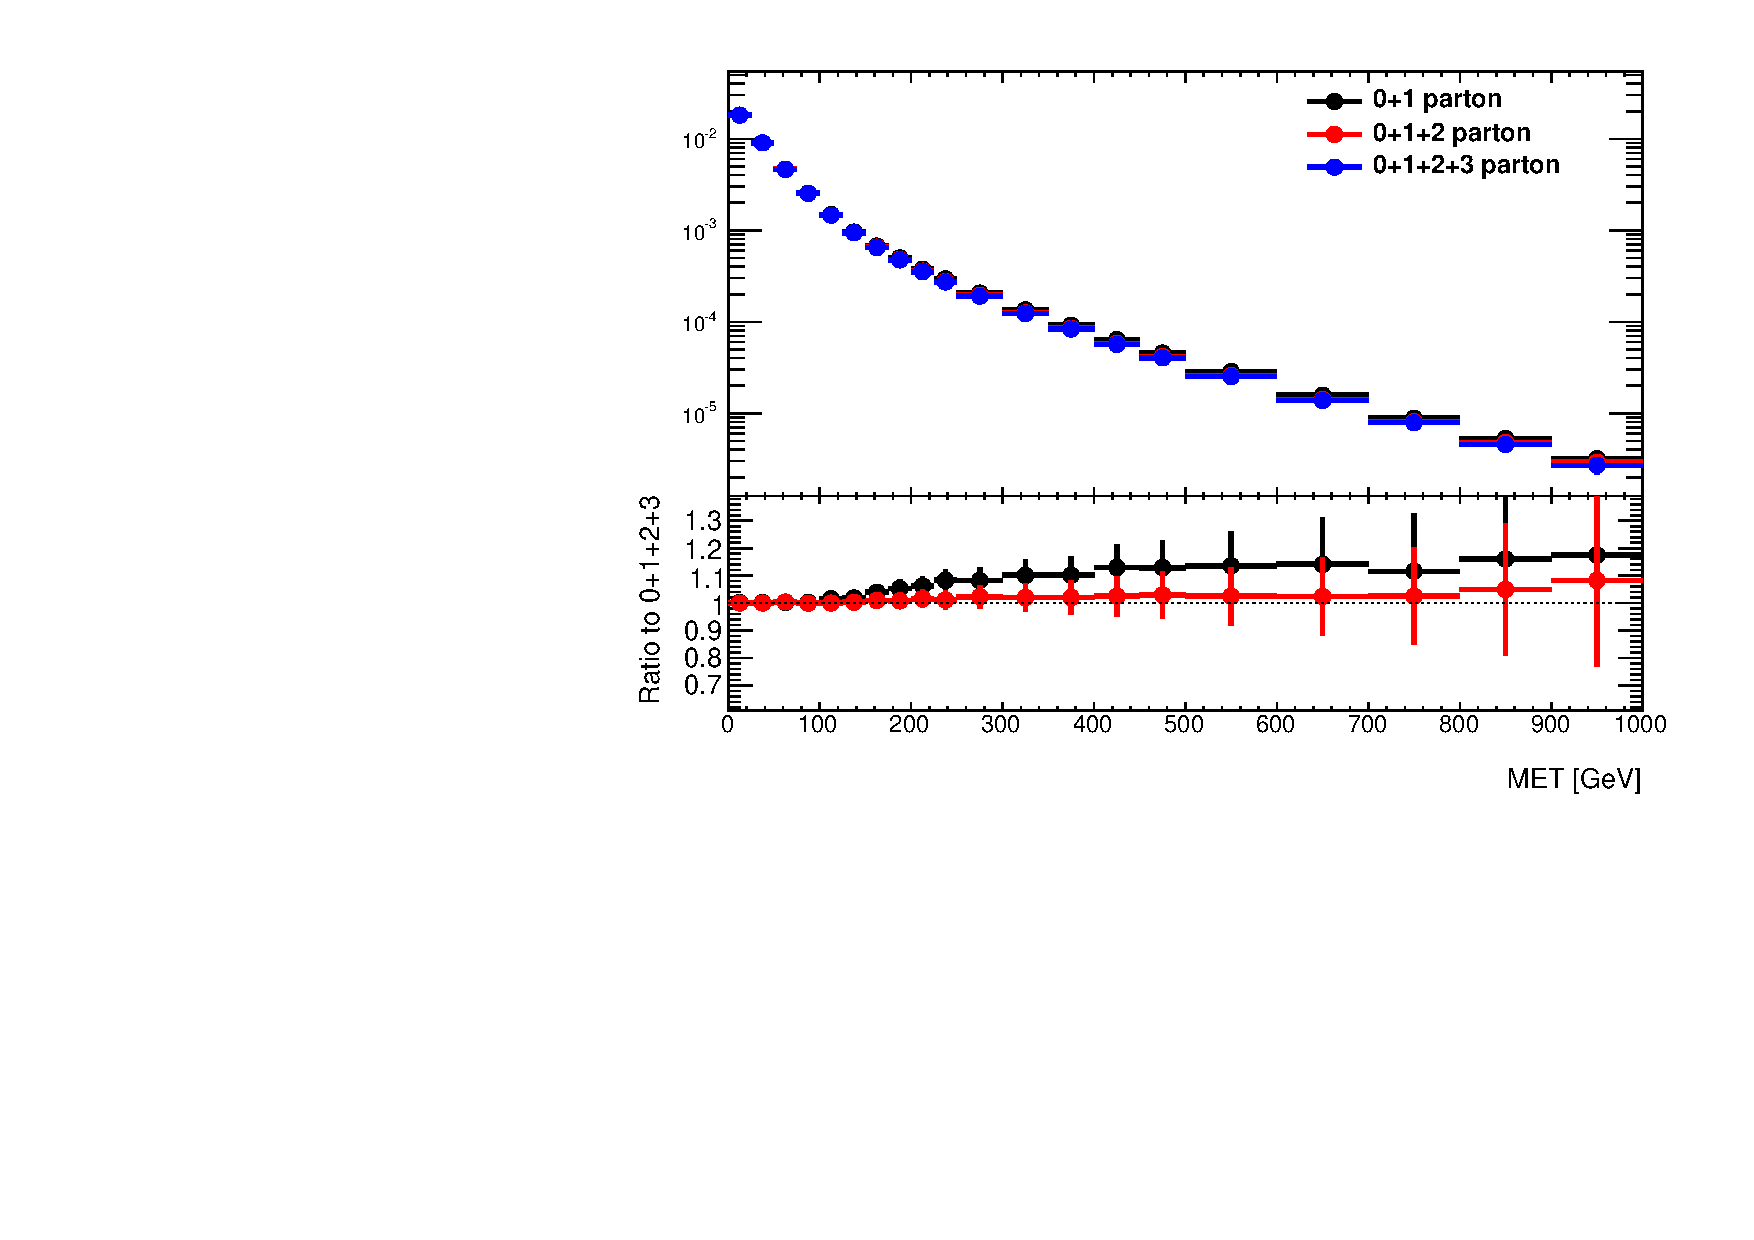
\includegraphics[width=0.95\linewidth]{figures/monojet_appendix/h_MET.pdf}
	}
	\hfill
	\subfloat[$N_{\text{jet}}\leqslant$3]{%
		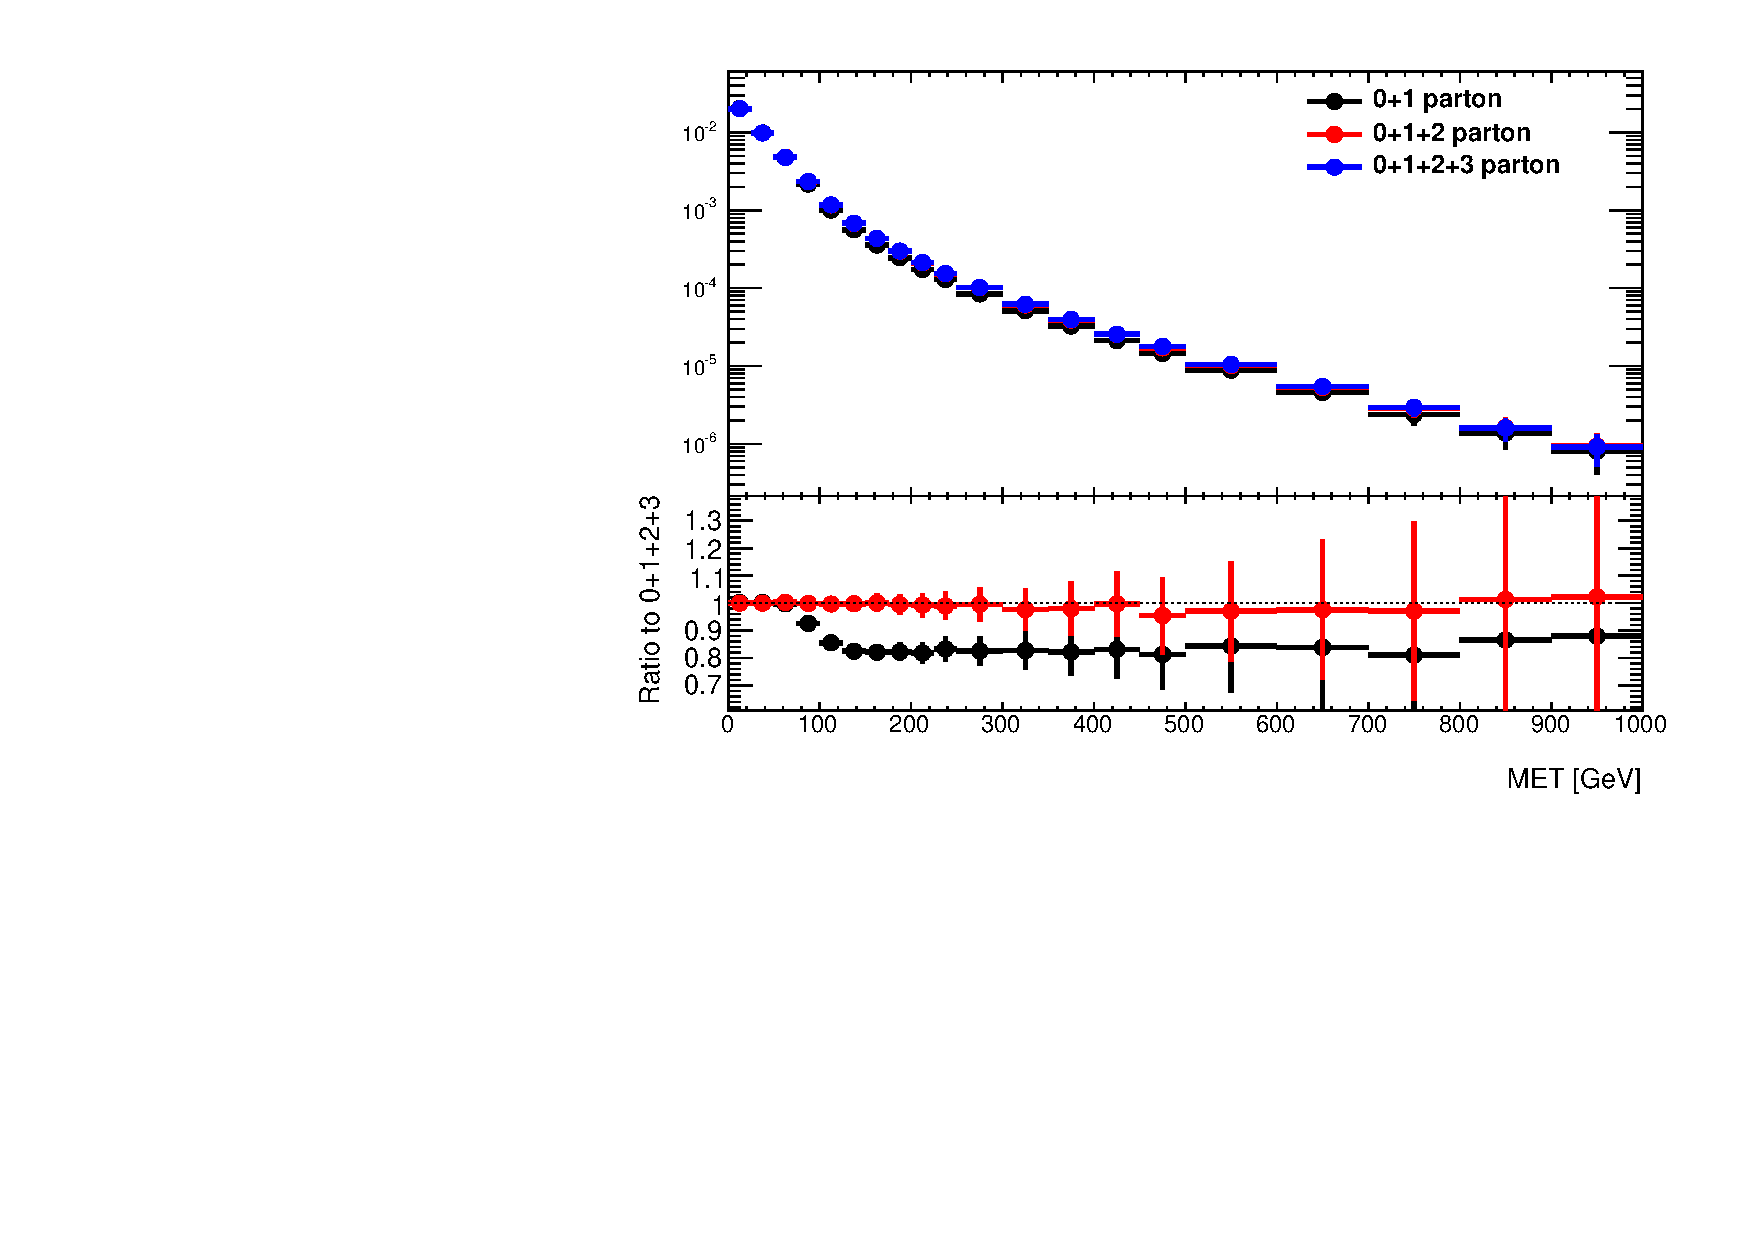
\includegraphics[width=0.95\linewidth]{figures/monojet_appendix/h_MET_3jet.pdf}
	}
	\hfill
%	\subfloat[Transverse momentum of subleading jet]{%
%		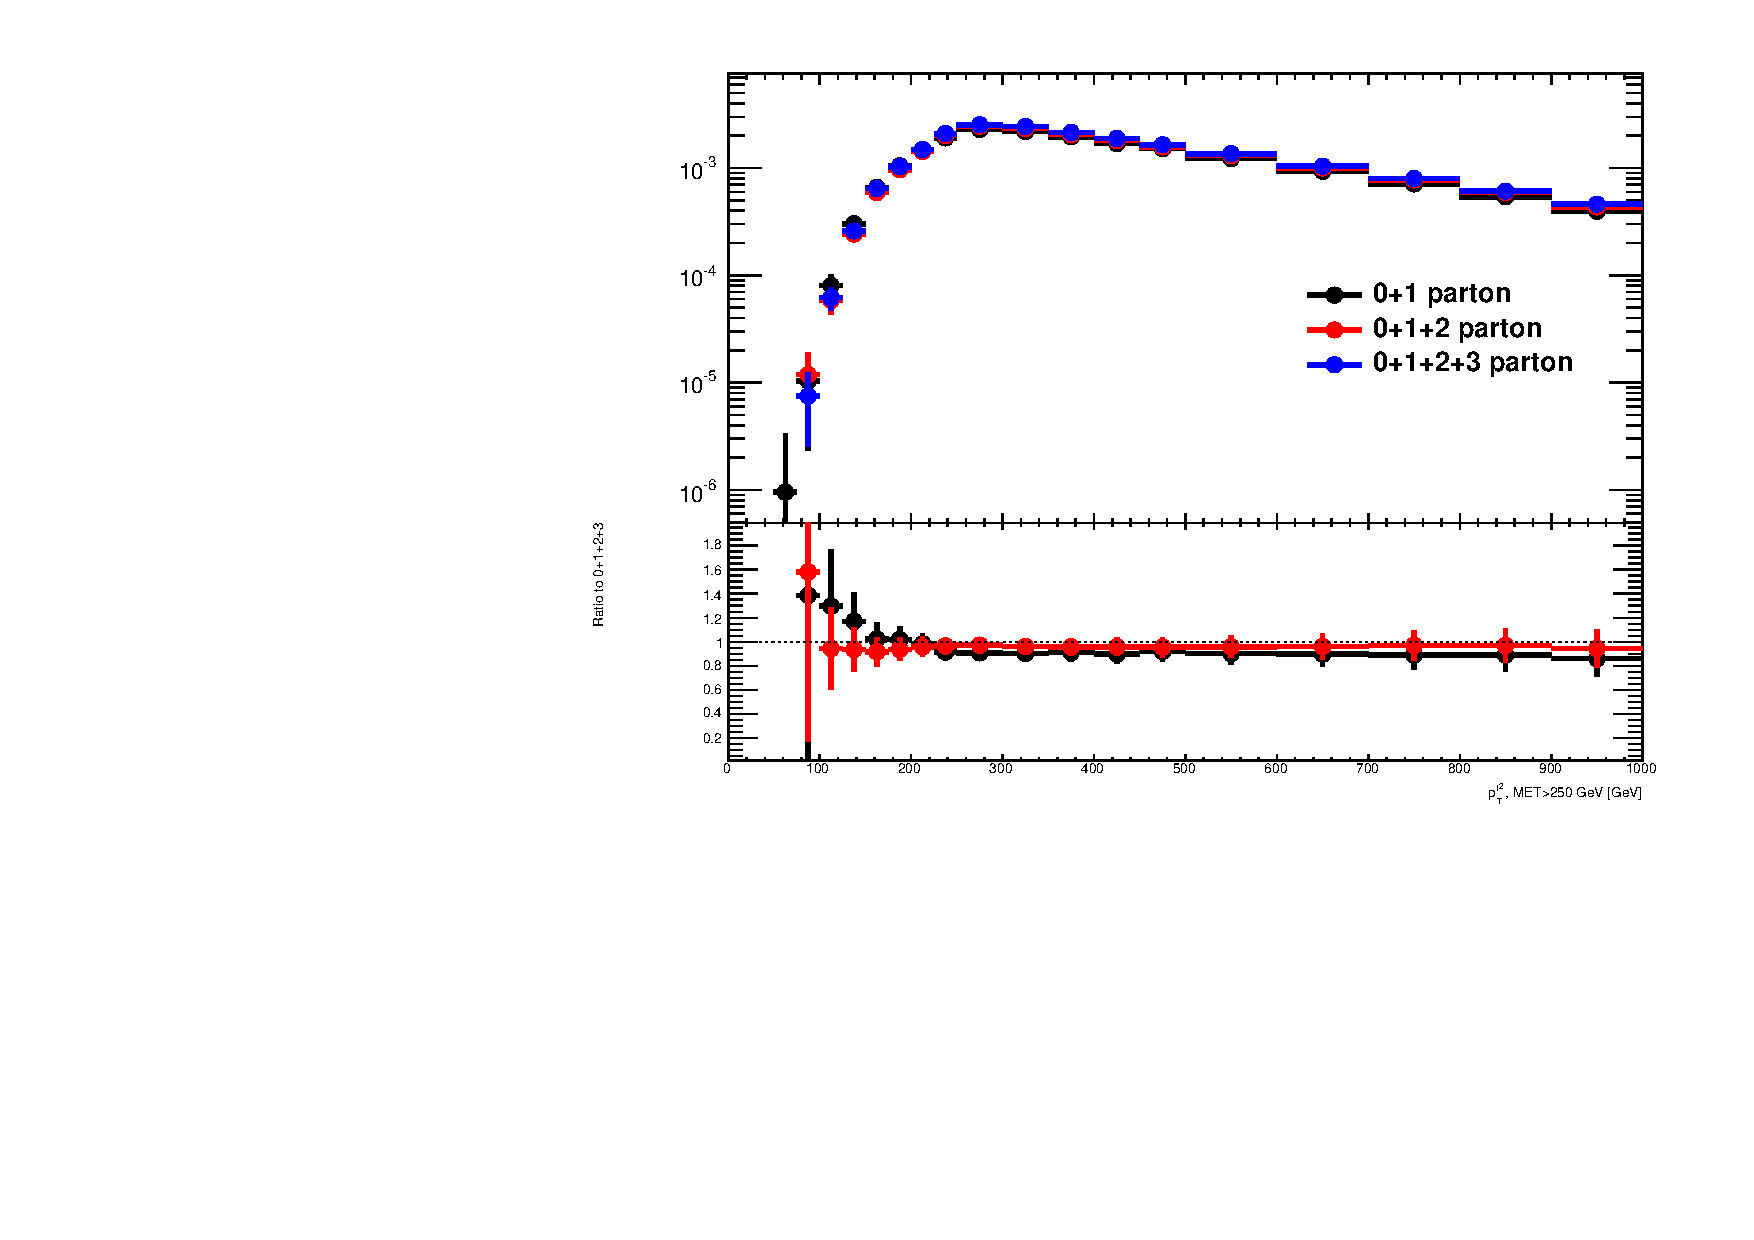
\includegraphics[width=0.95\linewidth]{figures/monojet_appendix/h_pt2_MET250.pdf}
%	}
%	\caption{Kinematics distributions for EFT D5 sample with CKKW matching scale at 80 \gev. 0-, 1-, 2- and 3-parton emission cases are generated separatedly and added together by cross sections.}
	\caption{Missing transverse momentum distributions for EFT D5 sample with CKKW-L matching scale at 80\,\gev produced with maximum 1 (black), 2 (red) and 3 (blue) partons emitted at the generator level. The ratios are shown with respect to the latter sample.}
	\label{fig:RatioKine_D5}
\end{figure}


\begin{figure}[h!]
	\centering  
%	\subfloat[Jet multiplicity, leading jet $p_{T}>30$ \gev]{%
%    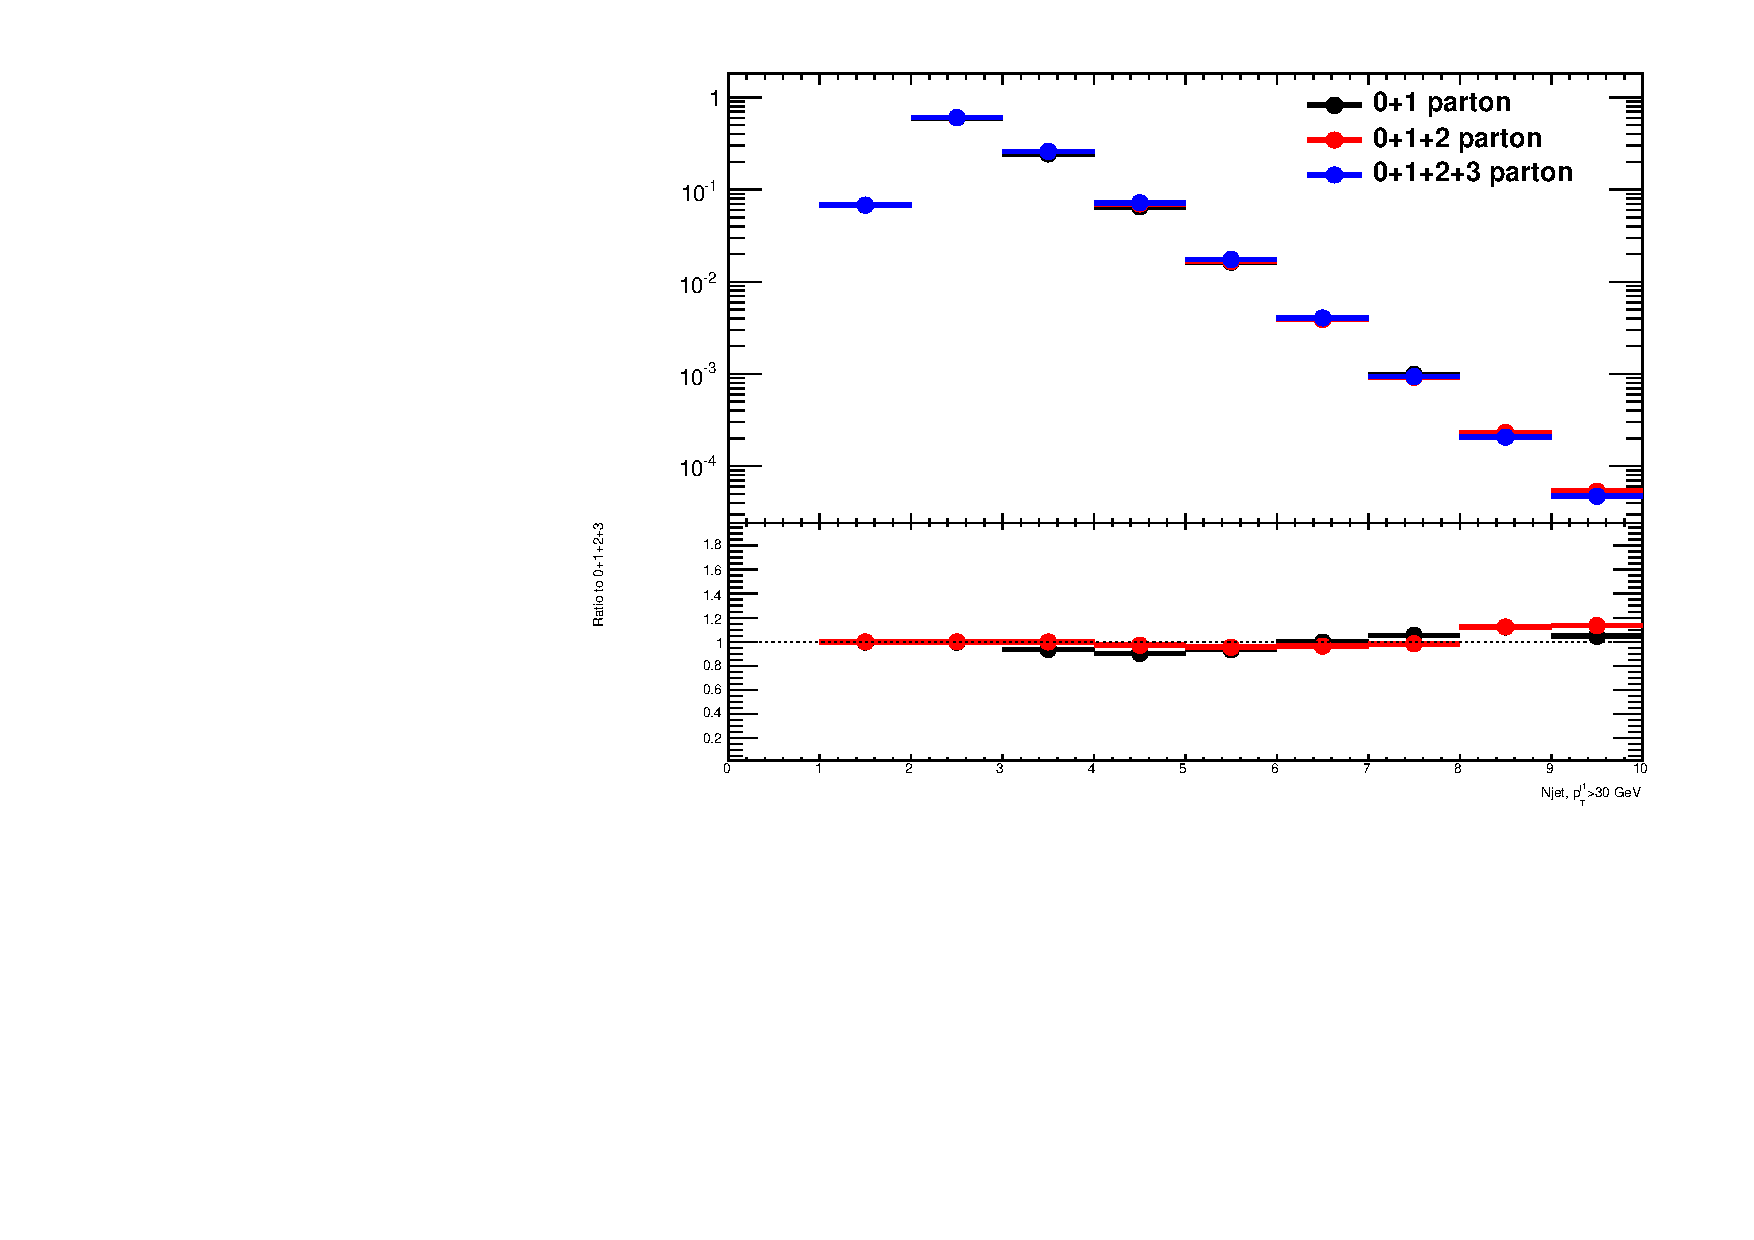
\includegraphics[width=0.95\linewidth]{figures/monojet_appendix/h_njet30.pdf}
%	}
%	\hfill
%	\subfloat[Jet multiplicity, leading jet $p_{T}>80$ \gev]{%
%    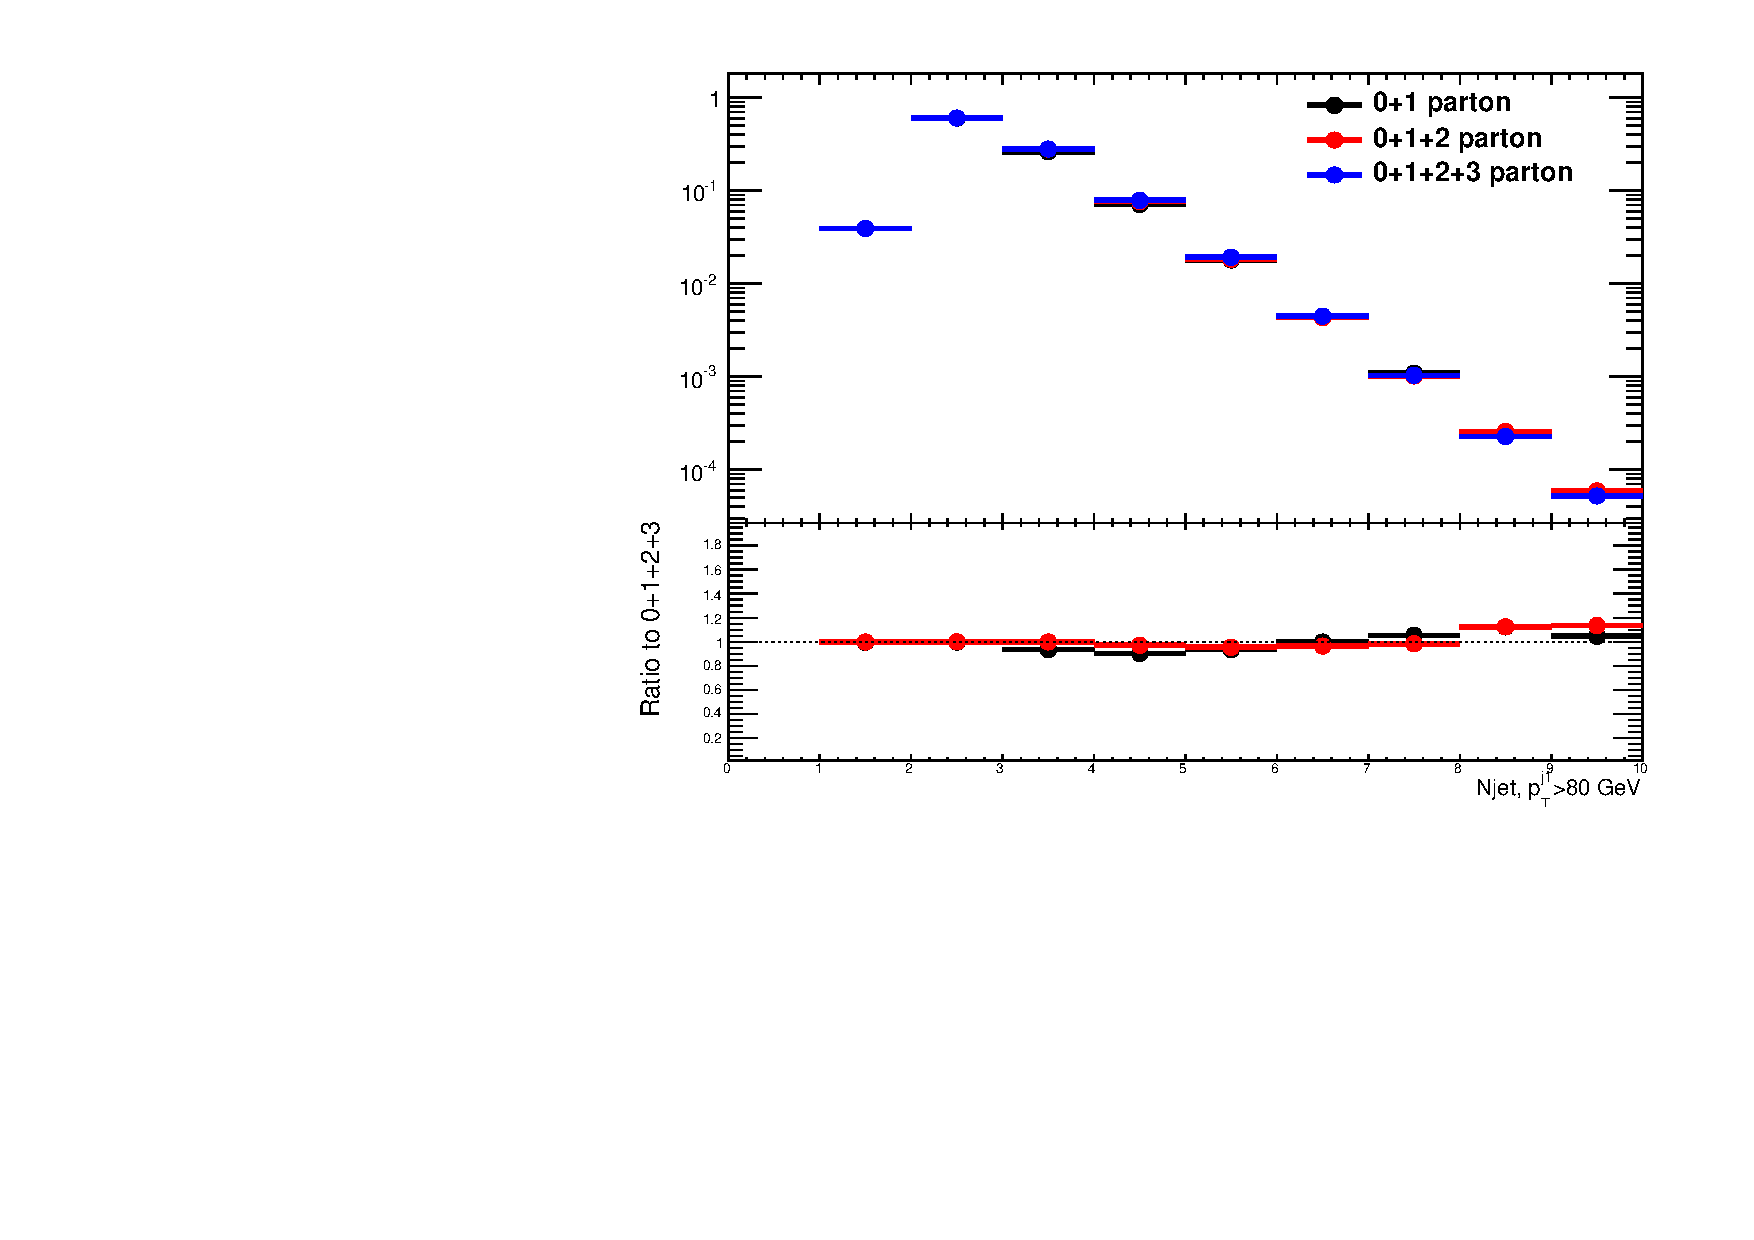
\includegraphics[width=0.95\linewidth]{figures/monojet_appendix/h_njet80.pdf}
%	}
%	\hfill
%	\subfloat[Jet multiplicity, leading jet $p_{T}>250$ \gev]{%
	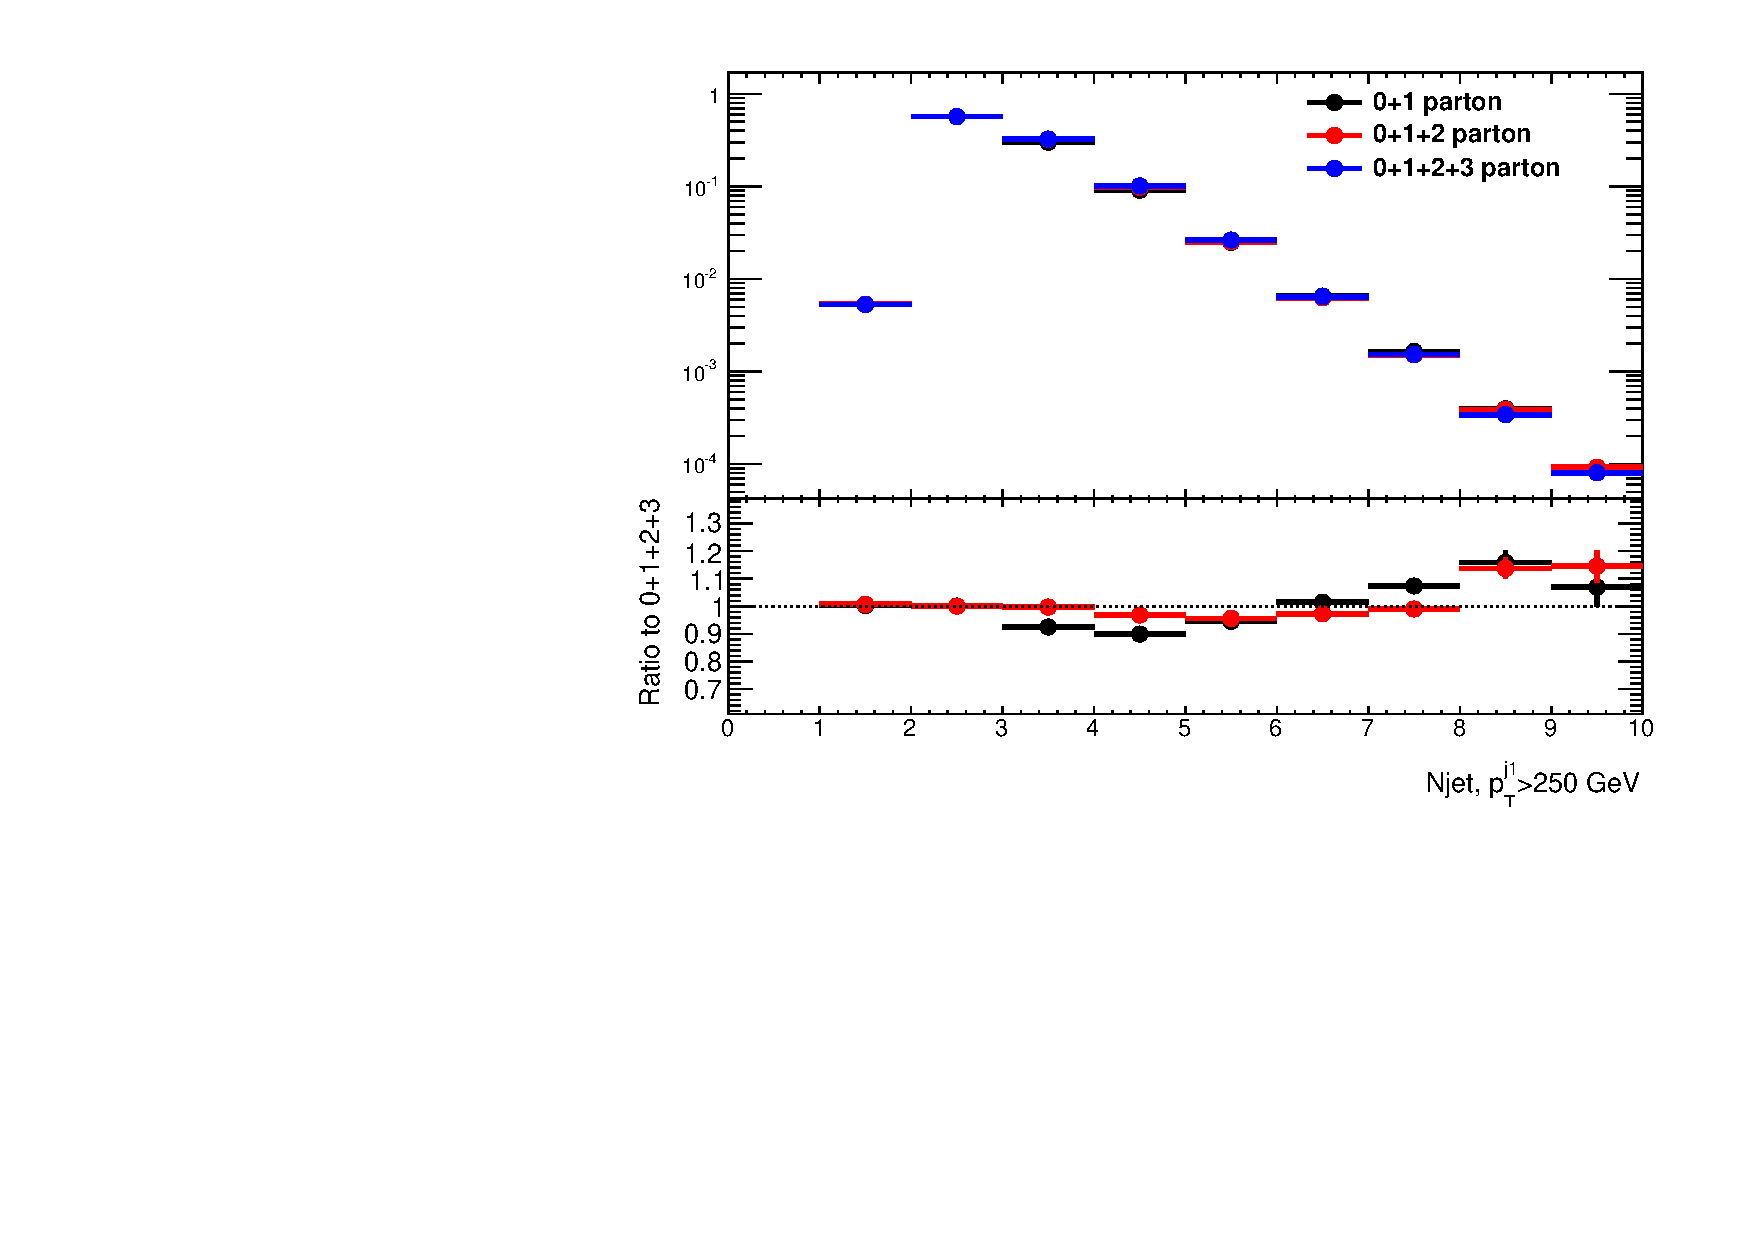
\includegraphics[width=0.95\linewidth]{figures/monojet_appendix/h_njet250.pdf}
%	}
%	\caption{Jet multiplicity distributions for EFT D5 sample with CKKW matching scale at 80 \gev. 0-, 1-, 2- and 3-parton emission cases are generated separatedly and added together by cross sections.}
	\caption{Multiplicity of jets with $\pT>30\,\gev$ and $|\eta|<2.8$ for EFT D5 sample with CKKW-L matching scale at 80\,\gev produced with maximum 1 (black), 2 (red) and 3 (blue) partons emitted at the generator level. The ratios are shown with respect to the latter sample. The leading jet $\pT$ is required to be larger than 250\,\gev.}
	\label{fig:RatioKine_D5_2}
\end{figure}

\subsection{Implementation of models for EW final states}
\label{sec:EW_implementation}

These models are generated at leading
order with \madgraph 2.2.2, using \pythiaEight for the parton shower.
Parameter cards can be found on the Forum SVN repository~\cite{ForumSVN_EW_DMV}.
No parton matching is currently implemented, since the visible signal comes from
the production of a heavy SM boson.   As a result, no special runtime configuration is needed
for \pythiaEight.

\subsection{\texorpdfstring{Implementation of models with heavy flavor quark signatures}{Implementation of models for heavy flavor quark signatures}}
\label{sec:TTBar_implementation}

The models for the $t \bar{t}$ and $b \bar{b}$ signatures are generated at leading
order with \madgraph 2.2.2, using \pythiaEight for the parton shower. No matching is currently
implemented.
Parameter cards can be found on the Forum SVN repository~\cite{ForumSVN_DMTTBar}.

We simulate the bFDM model at LO+PS using \madgraph v2.2.3 and \pythiaEight for the parton shower. 
Parton matching is needed in the case of the $b\bar{b}$+\MET{} final state, but it has not been
studied within the Forum. 
The corresponding card files can be found 
on the Forum SVN repository~\cite{ForumSVN_DMSingleB}.

\subsubsection{Quark flavor scheme and masses}

In this particular model we recommend an additional care when choosing
the flavor scheme generation and whether quarks should be treated as massive or massless. 

The production of DM+$b\bar{b}$, Dark Matter in association with $b$ jets via a decay of a (pseudo) scalar boson, 
is dominated in simplified mediator models by the gluon-gluon initiated production, similar to the production of 
Z+$b\bar{b}$ at the LHC. The Z+$b\bar{b}$ process has been studied in detail in the Z(ll)+$b$-jets final state, 
which can be used to validate both the modeling of DM+bb and, its main background, Z(vv)+$b\bar{b}$. 
In this context, the $p_\textrm{T}$ of the Z boson is related to the observed MET, whereas the $b$-jet kinematics 
determines the ratio of mono-$b$/di-$b$ signatures in the detector.

%suggestion: could add diagrams for Z+bb and Phi+bb production here%

For basic kinematic criteria applied to Z+$b\bar{b}$ production, this process leads in $\sim90\%$ of 
the events to a signature with only 1 $b$-jet in the acceptance ('Z+1$b$-jet production') and only in 
$\sim10\%$ of the events to a signature with 2 $b$-jets in the detector ('Z+2$b$-jets production). 
The production cross section of the Z+$b\bar{b}$ process are calculated in the 'five-flavor scheme', 
where b quarks are assumed massless, and the 'four-flavor scheme', where massive b quarks are 
used~\cite{Campbell:2003dd,Maltoni:2005wd,Campbell:2005zv}, 
and data favor the cross-section predictions in the five-flavor scheme~\cite{Chatrchyan:2014dha}.
We therefore recommend to calculate the cross sections of these
models in the 5-flavor scheme, as in the repository. 
The PDF used to calculate these cross section is NNPDF3.0 (lhaid 263000). 

It is found that the best modeling of two $b$-quarks final states is achieved using a 4-flavor scheme and a massive treatment of the $b$-quarks ~\cite{Chatrchyan:2014dha,Chatrchyan:2013zja,CMS:2015mba}. We recommend to use in the generation NNPDF3.0 set (lhaid 263400).
Since figure~\ref{fig:4Fvs5F} shows that there is no significant difference in the kinematics between 
either flavor scheme used for DM+$b\bar{b}$ production, we recommend the 4-flavor scheme to follow
the observation in the Z+$b\bar{b}$ measurements. 

%Table~\ref{tab:xsec_dmbb_g1} gives the production cross sections for all recommended samples with $g_\textrm{DM}=g_\textrm{SM}=1$.

% We recommend to use in the generation NNPDF3.0 set (lhaid
%263400).
%In the $t bar t$ case we provide 
%values for the suggested coupling scan. 

\begin{figure}[h!]
\begin{minipage}{0.49\textwidth}
	\centering 
	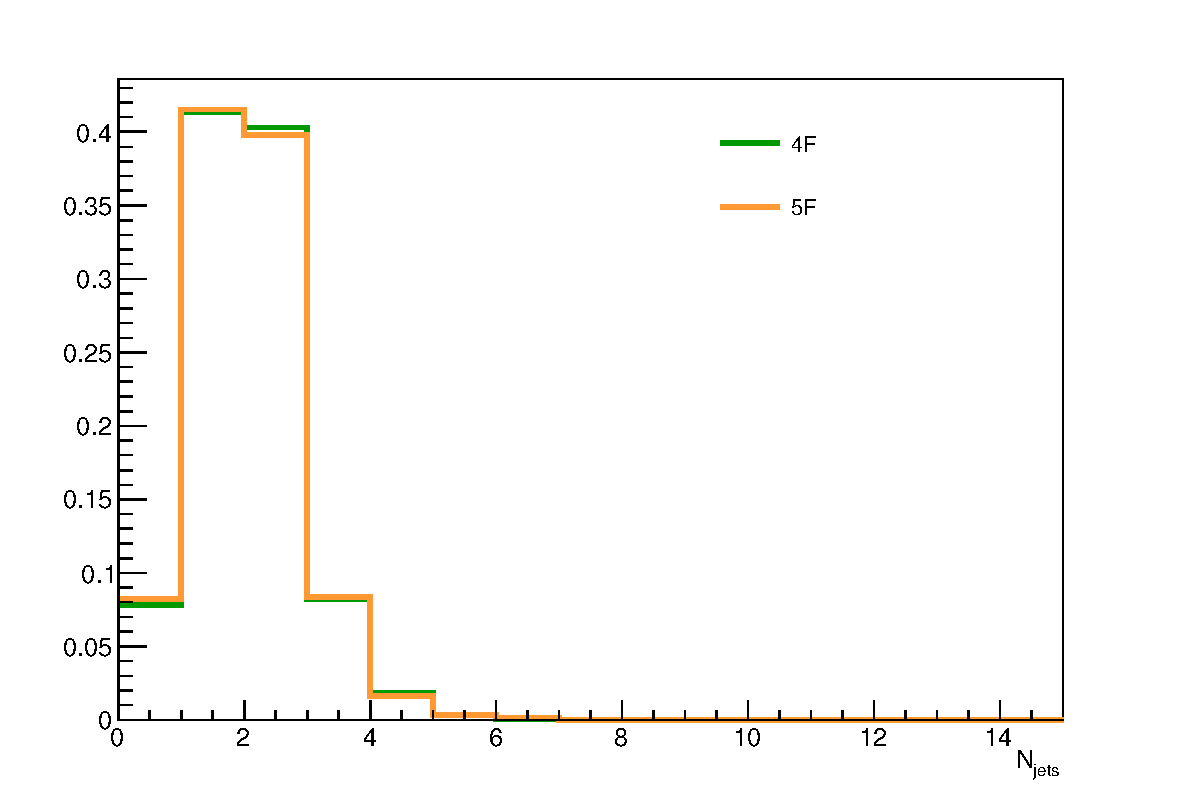
\includegraphics[scale=0.32]{figures/bbar/4Fvs5F_plots/Njets}
\end{minipage}
\hfill
\begin{minipage}{0.49\textwidth}
	\centering 
	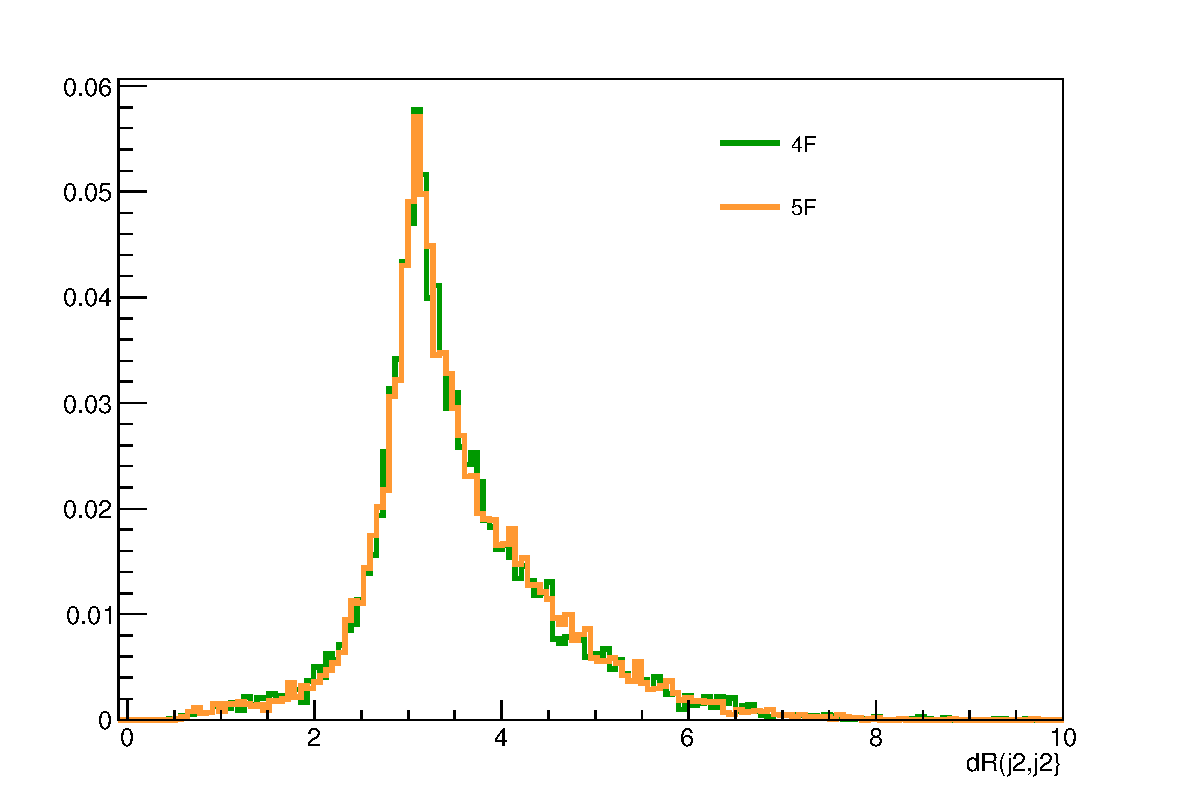
\includegraphics[scale=0.32]{figures/bbar/4Fvs5F_plots/dR12}
\end{minipage}
\caption{Comparison of the jet multiplicity (left) and angular correction $\Delta R(j_1, j_2)$ (right) for the DM+$b\bar{b}$ scalar model generated in the 4-flavor and 5-scheme.
	The samples are generated for $m_\chi=1$~GeV and $m_\phi=10$~GeV.
	\label{fig:4Fvs5F}}
\end{figure}

\section{\texorpdfstring{Implementation of specific models for $V+\MET$ analyses}{Implementation of specific models for V+MET analyses}}

\subsection{Model implementation for mono-Higgs models}
\label{sub:monoHiggs}

All three Higgs+\MET models are generated at leading
order with \madgraph 2.2.2, using \pythiaEight for the parton shower. No matching is needed. 
The \madgraph implementations of the scalar and vector models can be found on the Forum SVN 
repository~\cite{ForumSVN_EWMonoHiggs}, while the 2HDM model can be found
at this link~\cite{ForumSVN_EWMonoHiggs_2HDM}.

In all cases, it is recommended not to handle the $h$ decay through \madgraph as
it does not include the proper $h$ branching ratios, or, if using \madgraph, then the 
resulting cross section should be rescaled to match onto the correct branching ratio.

\subsubsection{\madgraph details for scalar mediator Higgs+MET model}

In this model, the contribution from the $gghS$ box is included through an effective 
Lagrangian evaluated in the large $m_t$ limit. 
This may overestimate the rates of the $h + \MET$ signal~\cite{Haisch:2012kf}, but a full evaluation
is left to future studies. 

\subsubsection{\madgraph details for 2HDM Higgs+MET model}
  
 The two couplings that can be changed in the implemented model follow the nomenclature below:
 \begin{itemize}
 	\item \texttt{Tb} - $\tan \beta$
 	\item \texttt{gz} - $g_z$, gauge coupling of \Zprime to quarks
 \end{itemize}
 The other couplings are not changed, including \texttt{gx} (the $A \bar \chiDM \chiDM$ coupling) which has little impact on the signal. 
 $\sin \alpha$ is fixed internally such that $\cos (\beta-\alpha) = 0$. 
 The width of the \Zprime and $A$ can be computed automatically within \madgraph. 
 The couplings here don't affect the signal kinematics, so they can be fixed to default values 
 and then the signal rates can be scaled appropriately. 
 
The nomenclature for the masses in the implemented model is:
 \begin{itemize}
 	\item \texttt{MZp} - PDG ID 32 - \Zprime
 	\item \texttt{MA0} - PDG ID 28 - $A$
 	\item \texttt{MX} - PDG ID 1000022 - dark matter particle
 \end{itemize}
 
The other masses are unchanged and do not affect the result. 
 Both $\Zprime \to hZ(\bar \nu \nu)$ and  $\Zprime \to hA(\bar \chiDM \chiDM)$ contribute to the final state, scaling
 different with model parameters. We recommend to generate them separately, 
 and then add the two signal processes together weighted by cross sections.
 % These signals should be generated separately since they have different $\tan \beta, M_A$ dependence.  

\subsection{Implementation of EFT models}
\label{sub:EFTModels}

These models are generated at leading
order with \madgraph 2.2.2, using \pythiaEight for the parton shower. No matching is currently
implemented.
Parameter cards can be found on the Forum SVN repository:~\cite{ForumSVN_EWMonoHiggs}
for operators with Higgs+MET final states
and ~\cite{ForumSVN_EWEFTD7} for $W/Z/\gamma$ final states.

